
\documentclass[11pt,fleqn]{article}
\usepackage[margin=1in,top=1in,bottom=1in]{geometry}
\usepackage{mathtools}
\usepackage{longtable}
\usepackage{enumitem}
\usepackage{hyperref}
\usepackage[dvips]{graphics}
\usepackage[table]{xcolor}
\usepackage{amssymb}
\usepackage{subfig}
\usepackage{booktabs}

\usepackage[normalem]{ulem}

\usepackage{multicol}
\usepackage{txfonts}
%\usepackage{amsfonts}
\usepackage{natbib}
\usepackage{gb4e}
%\usepackage{/Users/judith/Library/Latex/drs}
%\usepackage{/Users/judith/Library/Latex/avm}
\usepackage[all]{xy}
\usepackage{rotating}
\usepackage{tipa}
\usepackage{multirow}
\usepackage{authblk}


\newcommand{\foc}{$_{\mbox{\small F}}$}
\newcommand{\lp}{<_{\hspace*{-.1cm}p}}
\newcommand{\lnai}{<_{\hspace*{-.1cm}nai}}

\setlength{\parindent}{.8cm}
\setlength{\parskip}{0ex}
\setlength{\headsep}{0in}

\setlength{\bibsep}{0mm}
\bibpunct[:]{(}{)}{;}{a}{,}{,}

\newcommand{\yi}{\'{\symbol{16}}}
\newcommand{\nasi}{\~{\symbol{16}}}
\newcommand{\hina}{h\nasi na}
\newcommand{\ina}{\nasi na}
%\renewcommand{\abut}{$\supset$\hspace*{-0.07cm}$\subset$}
\newcommand{\tto}{t$_{top}$}
\newcommand{\wtop}{w$_{top}$}
\newcommand{\tc}{t$_c$}
\newcommand{\schwa}{\begin{sideways}e\end{sideways}}

% Semantic brackets
%\newcommand{\iss}[1]{\mbox{\protect\tiny \mbox{#1}}}
%\newcommand{\sem}[2]{\6#1\9$_\iss{#2}$} David's original
\newcommand{\6}{\mbox{$[\hspace*{-.6mm}[$}} 
\newcommand{\9}{\mbox{$]\hspace*{-.6mm}]$}}
\newcommand{\sem}[2]{\6#1\9$^{#2}$}

\newcommand{\semt}[2]{$\left[\hspace*{-.6mm}\left[\begin{tabular}[c]{@{}l@{}}#1\vspace*{-.5em}\end{tabular}\right]\hspace*{-.6mm}\right]\hspace*{-.6mm}^{#2}$}

%\renewcommand{\baselinestretch}{1.2}

\def\bad{{\leavevmode\llap{*}}}
\def\marginal{{\leavevmode\llap{?}}}
\def\verymarginal{{\leavevmode\llap{??}}}
\def\infelic{{\leavevmode\llap{\#}}}

\definecolor{Lighter}{gray}{.92}
\definecolor{Blue}{RGB}{0,0,255}
\definecolor{Green}{RGB}{10,200,100}
\definecolor{Red}{RGB}{255,0,0}


\newcommand{\citepos}[1]{\citeauthor{#1}'s \citeyear{#1}}
\newcommand{\citeposs}[1]{\citeauthor{#1}'s}
\newcommand{\citetpos}[1]{\citeauthor{#1}'s (\citeyear{#1})}

\newcommand{\eref}[1]{(\ref{#1})}
\newcommand{\tableref}[1]{Table \ref{#1}}
\newcommand{\figref}[1]{Fig.~\ref{#1}}
\newcommand{\appref}[1]{Appendix \ref{#1}}
\newcommand{\sectionref}[1]{Section \ref{#1}}


\title{Information-structure as a source of projection variability}

\author[$\bullet$]{Judith Tonhauser}
\author[$\circ$]{David Beaver}
\author[$\triangleright$]{Judith Degen}


\affil[$\bullet$]{The Ohio State University}
\affil[$\circ$]{University of Texas at Austin}
\affil[$\triangleright$]{Stanford University}


\renewcommand\Authands{ and }

\newcommand{\jt}[1]{\textbf{\color{blue}JT: #1}}
\newcommand{\jd}[1]{\textbf{\color{blue}[jd: #1]}}  

\begin{document}

\maketitle

\begin{abstract}
Projective content is utterance content that a speaker may be taken to be committed to it even when the expression that contributes the content occurs embedded under an entailment-canceling operator (e.g., \citealt{ccmg90}). Conventionalist approaches to projection assume that the projectivity of projective content derives from a conventionally specified requirement of such content to be entailed by or satisfied in the common ground of the interlocutors (e.g., \citealt{heim83,vds92}). An empirical challenge for such approaches to projection comes from the observation that projective content varies in how robustly it projects (e.g., \citealt{karttunen71b,simons01,abusch10}). An alternative approach, advanced in \citealt{brst-salt10}, maintains that projective content projects if and only if it is not at-issue with respect to the Question Under Discussion (\citealt{roberts12}) addressed by the utterance that contributes the projective content (see also \citealt{brst-ar}). Under this approach, projection variability can be attributed to variable at-issueness. This paper reports the findings of two pairs of experiments designed to explore the robustness with which projective content contributed by a wide range of English expressions projects and to test \citetpos{brst-salt10} hypothesis that the information-structural status of projective content influences projectivity. The two experiments provide robust empirical evidence for projection variability and, crucially, suggest that both the projective content trigger and the information-structural status of projective content influences the projectivity of projective content. The paper concludes by discussing the implications of these findings for an empirically adequate analysis of projective content.

\end{abstract}

%\tableofcontents

%\newpage
			
\section{Introduction}\label{s1}

Projective content is utterance content that the speaker may be taken to be committed to even when the expression that contributes the content occurs in the syntactic scope of an entailment-canceling operator (see, e.g., \citealt{ccmg90}). The speaker of (\ref{eng1}), for instance, is taken to be committed to the content of the complement of {\em discover}, that Mike visited Alcatraz, since this content is entailed by the utterance. The so-called Family-of-Sentences variants of (\ref{eng1}) given in (\ref{eng2}a-d) do not entail this content because {\em discover} is embedded under entailment-canceling operators: negation in (\ref{eng2}a), the polar question operator in (\ref{eng2}b), the epistemic possibility modal {\em perhaps} in (\ref{eng2}c) and the antecedent of a conditional in (\ref{eng2}d). Since speakers who utter the sentences in (\ref{eng2}a-d) may nevertheless be taken to be committed to the content of the complement, this content, by virtue of being able to `project' over the entailment-canceling operators, is considered projective content. 

\begin{exe}
\ex\label{eng1}  Felipe discovered that Mike visited Alcatraz.

\ex\label{eng2}
\begin{xlist} 
\ex Felipe didn't discover that Mike visited Alcatraz.
\ex Did Felipe discover that Mike visited Alcatraz?
\ex Perhaps Felipe discovered that Mike visited Alcatraz.
\ex If Felipe discovered that Mike visited Alcatraz, he'll get mad.
\end{xlist}
\end{exe}

Why does projective content project? According to mainstream approaches, projective content projects because it is conventionally specified to do so, for instance, by being required to be entailed by or satisfied in the common ground of the interlocutors (e.g., \citealt{heim83,vds92,geurts99}). On such `conventionalist' approaches, the lexical entry of {\em discover} specifies that the content of its clausal complement is required to be entailed by or satisfied in the common ground of the interlocutors, thereby ensuring that the speaker is taken to be committed to the content. Since conventionalist approaches only distinguish projective and non-projective content, such approaches are challenged by the long-standing observation that some projective content projects less robustly than other such content. In the early 1970s already, \citet{karttunen71b} pointed out that the content of the complement of {\em regret} in (\ref{semi-factive}a) is more robustly projective than the content of the complement of {\em discover} in (\ref{semi-factive}b); following \citealt{karttunen71b}, predicates like {\em discover} have since been referred to as `semi-factive', in contrast to their `factive' counterparts like {\em regret} (and `non-factive' predicates like {\em believe}). In \citealt{schlenker10}, the predicate {\em announce} was referred to as a `part-time trigger' because the content of its complement may, but often does not, project.

\begin{exe}
\ex\label{semi-factive}
\begin{xlist}
\ex John didn't discover that he had not told the truth.  
\ex John didn't regret that he had not told the truth.
\hfill (\citealt[63]{karttunen71b})

\end{xlist}
\end{exe}

Similarly, \citet[432]{simons01} noted, partially based on examples from \citealt{ccmg90} and \citealt{geurts94}, that the projection of ``some -- but crucially, not all'' projective content to the common ground of the interlocutors may be suppressed in explicit ignorance contexts. Example (\ref{hardsoft}a), for instance, shows that the projective content of {\em win} in the antecedent of the conditional, that John participated in the race, need not be part of the common ground of the interlocutors, i.e., need not project. On the other hand, the existential implication of the cleft in (\ref{hardsoft}b), that there is an individual who read the letter, must be part of the common ground of the interlocutors, i.e., must project. Expressions like {\em win} are referred to as `soft triggers', in contrast to `hard triggers', like the cleft (see also, e.g., \citealt{abusch10}).

\begin{exe}
\ex\label{hardsoft}
\begin{xlist}

\ex I have no idea whether John ended up participating in the Road Race yesterday. But if he won it, then he has more victories than anyone else in history. \hfill (\citealt[39]{abusch10})

\ex\infelic I have no idea whether anyone read that letter. But if it is John
who read it, let's ask him to be discreet about the content. \hfill (\citealt[40]{abusch10})

\end{xlist}
\end{exe}

Experimental research has also provided preliminary evidence for projection variability. \citet{xue-onea11} observed that the content of the complement of German {\em wissen} `know' is less projective than the content of the complement of {\em erfahren} `find out', both of which are less projective than the relevant projective contents of sentences with {\em auch} `too' (that a parallel event is contextually salient) and {\em wieder} `again' (that the relevant event has happened before). Similarly, \citet{smith-hall11} found that the projective contents of {\em win} and {\em know} are less projective than the content implication of English definite noun phrases (e.g., for {\em the queen}, that the referent is a queen). Interestingly, they also found that the existential implication of cleft sentences, considered a hard trigger, was (numerically) less projective than the relevant contents of the soft triggers {\em win} and {\em know}. Thus, the (sparse) experimental evidence confirms some but not all of the intuitions about projection variability reported in the literature.\footnote{\citet{tiemann-etal11} noted that presuppositions differ in how acceptable they were judged to be in contexts that did not entail the relevant content, but projection variability was not the focus of their paper.}

Observations about projection variability challenge conventionalist approaches to projection because such approaches do not offer an explanation for why some projective content seems to systematically project less robustly than other such content. After all, under such approaches, any expression that contributes projective content lexically specifies that the relevant content is required to be entailed by or satisfied in the common ground of the interlocutors. The lexical specifications of expressions like {\em regret, discover, win}, clefts and definite noun phrases thereby predict that their relevant contents can project, but do not predict differences in how robustly the contents project. Referring to triggers of projective content as `semi-factive' or `soft', as opposed to `factive' or `hard', serves to remind of projection variability but does not address the challenge that this variability poses for conventionalist approaches to projection.

One possible explanation for projection variability is that projectivity derives from a property that projective content shares, but shares to varying degrees. \citet{brst-salt10} proposed that this property is `at-issueness', i.e., the ability of content to address the Question Under Discussion (QUD; e.g., \citealt{roberts12}).  Specifically, Simons and her colleagues proposed that utterance content projects if and only if it is not at-issue with respect to the QUD addressed by the utterance. This hypothesis is formulated as the Projection Principle in \citealt[280]{brst-ar}:

\begin{exe}
\ex\label{pp} {\bf Projection Principle:} If content $C$ is expressed by a constituent embedded under an entailment-canceling operator, then $C$ projects if and only if $C$ is not at-issue.

\end{exe} 
Although Simons and her colleagues did not consider projection variability, the Projection Principle predicts such variability. For instance, their proposal predicts that the content of non-restrictive relative clauses (NRRCs) projects more robustly, by virtue of being not at-issue (\citealt{potts05}), than the content of the complement of {\em discover}, which can be at-issue and not-at-issue (\citealt{simons07}). Consider the question-answer pairs in (\ref{nrrc}): the example in (\ref{nrrc}a) shows that the content of the NRRC in B's utterance cannot be used to address A's question, and hence is not at-issue; the example in (\ref{nrrc}b) shows that the main clause content of B's utterance can address A's question and hence is at-issue. The content of the complement of {\em discover}, on the other hand, can be not-at-issue, as shown in (\ref{discover}a), but it can also be at-issue, as shown in (\ref{discover}b).\footnote{\citet{syrett-koev2015} show that the content of NRRCs can be the target of direct denial, which may be taken to suggest that this content can be at-issue. We return to this matter in section \ref{s5}.} Thus, if the content of NRRCs is more robustly not-at-issue than the content of the complement of {\em discover}, the former is predicted by \citetpos{brst-salt10} proposal to project more robustly than the latter. 

\begin{exe}
\ex\label{nrrc}
\begin{xlist}
\ex
\begin{xlist}
\exi{A:} Did Mike visit Alcatraz?
\exi{B:} \infelic Mike, who visited Alcatraz, is interested in the history of prisons.
\end{xlist}


\ex
\begin{xlist}
\exi{A:} What is Mike interested in?
\exi{B:} Mike, who visited Alcatraz, is interested in the history of prisons.
\end{xlist}


\end{xlist}

\ex\label{discover}
\begin{xlist}

\ex
\begin{xlist}
\exi{A:} Why is Henry in such a bad mood?
\exi{B:} He discovered that Harriet had a job interview at Princeton. 
\end{xlist}

\ex
\begin{xlist}
\exi{A:} Where was Harriet yesterday?
\exi{B:} Henry discovered that she had a job interview at Princeton. \hfill (\citealt[1035]{simons07})
\end{xlist}
\end{xlist}
\end{exe}

This paper has two goals, which are explored on the basis of two pairs of experiments. The first goal (Experiments 1a and 1b) is to explore projection variability for a broad range of projective content, to better understand the extent to which projective content varies in its projectivity. The second goal (addressed through Experiments 1a and 1b, as well as Experiments 2a and 2b) is to test a prediction of the Projection Principle, namely that the at-issueness of projective content is inversely correlated with its projectivity. These two goals jointly serve to identify the empirical generalizations that an empirically adequate analysis of projection needs to account for. 

In pursuing our first goal, we expand on and improve on previous experimental research on projection variability. In \citealt{xue-onea11} and \citealt{smith-hall11}, projection variability was explored for 4 German and 6 English expressions that contribute projective content, respectively. Experiments 1a and 1b significantly broaden our understanding of projection variability by considering the projective content of 19 expressions (which are introduced in section \ref{s2}). Our experiments also take into consideration that lexical content may influence projection: a speaker might, for instance, be more likely to be taken to be committed to the content that Alexander flew to New York than to the content that Alexander flew to the moon, simply because people are more likely to fly to New York than the moon. In other words, the lexical content that instantiates the projective content of an expression\footnote{\label{f-content}In this paper, we use `lexical content' to refer to the content of an expression and `projective content' to refer to an abstract characterization of the projective content of an expression. For instance, in B's utterance in (\ref{discover}a), the relevant expression is {\em discover}, the projective content is the content of its clausal complement, and the lexical content (of the projective content) is that Harriet had a job interview at Princeton.} may matter for how robustly the projective content is taken to be a commitment of the speaker and how likely the projective content is to address the QUD. The projective content of the 6 expressions explored in \citealt{smith-hall11} was only instantiated by one lexical content each and a distinct lexical content instantiated each projective content. Our experiments, in contrast, included a total of 37 lexical contents and the projective content of each expression was instantiated by up to 20 lexical contents. Furthermore, to facilitate comparison across the different projective contents (and the expressions that contribute them), the projective contents of distinct expressions were instantiated with the same lexical contents: overall, each of the 37 lexical contents instantiated up to 12 projective contents.

Our second goal -- to test the Projection Principle -- also builds on and significantly expands previous experimental work. 
 Using a direct dissent diagnostic for at-issueness, \citet{amaral-etal11} found that speakers of British English judged direct dissent with the projective content of {\em only} (the prejacent) to be more acceptable than direct dissent with the projective content of {\em continue} and {\em stop} (the pre- and post-state implications, respectively). These findings suggest that the prejacent of {\em only} is more at-issue than the post- and pre-state implications of {\em continue} and {\em stop}. (See also \citealt{cummins-etal2012}, and \citealt{amaral-cummins2015} for similar results on Spanish.) \citet{xue-onea11} found that speakers of German were more likely to directly dissent with the content of the complement of {\em wissen} `know' than with the content of the complement of {\em erfahren} `find out' and, in turn, more likely to directly dissent with these contents than with projective contents of {\em auch} `too' and {\em wieder} again'. These results suggest that the projective content of {\em wissen} `know' is more at-issue than the projective content of {\em erfahren} `find out', which in turn are comparatively more at-issue than the projective contents of {\em auch} `too' and {\em wieder} again'. Interestingly, comparing the relative projectivity and not-at-issueness 
of the projective contents across their two experiments, \citet[180]{xue-onea11} point to ``a clear correlation between projection and not-at-issueness'', in line with the Projection Principle that we explore further here. Our Experiments 1a and 1b improve on \citetpos{xue-onea11} study by exploring the projectivity and the not-at-issueness of projective content as within-item and within-participant factors. The design of these experiments therefore allows us to quantify the correlation between not-at-issueness and projectivity, and to assess by-item and by-participant variability. Since different diagnostics have been used in the literature to diagnose (not-)at-issueness (for discussion, see, e.g., \citealt{tonhauser-sula6} and section \ref{s3}), the second pair of experiments, Experiments 2a and 2b, explore the not-at-issueness of the projective contents of the first pair of experiments, Experiments 1a and 1b, using a different diagnostic for at-issueness. The results of the two pairs of experiments thus also allow for a comparison of two diagnostics for at-issueness.

The paper proceeds as follows. In section \ref{s2}, we characterize the projective contents explored in this paper. Section \ref{s3} addresses the two goals of the paper on the basis of Experiments 1a and 1b, and section \ref{s4} extends our investigation of the second goal on the basis of Experiments 2a and 2b. In section \ref{s5}, we discuss the implications of our findings for analyses of projection. Section \ref{s6} concludes the paper.

\section{The projective contents explored in the experiments}\label{s2}

The projective contents associated with 19 target expressions are explored in the two pairs of experiments. The projective content associated with the 9 target expressions in Experiment 1a are syntactically heterogeneous, as shown in (\ref{pairs1a2a}), whereas the 12 target expressions included in Experiment 1b are all (semi-)factive attitude predicates, as shown in (\ref{pairs1b2b}). Since some expressions can contribute multiple projective contents (\citealt{brst-lang11}), we specify, for each target expression, the projective content investigated in our experiments: e.g., in (\ref{pairs1a2a}a), `sentence-medial NRRCs' identifies the target expression and `content of the NRRC' identifies the projective content. Experiments 2a and 2b explored not-at-issueness for the same expression/projective content pairs as Experiments 1a and 1b, respectively. Since the projective content of the attitude predicates {\em annoyed} and {\em discover} was explored in both pairs of experiments, a total of 19 expression/projective content pairs were explored. 

\begin{exe}
\ex\label{pairs1a2a} {\bf Expression/projective content pairs in Experiments 1a and 2a}

\begin{enumerate}[itemsep=-.5mm]

\item Sentence-medial NRRCs / content of the NRRC
\\ e.g., {\em Martha, who has a new BMW, drives fast}; content: `Martha has a new BMW'

\item Sentence-medial nominal appositives / appositive content
\\ e.g., {\em Martha's new car, a BMW, was expensive}; content: `Martha has a BMW'

\item Posessive noun phrases / possession implication
\\ e.g., {\em Martha's new car is a BMW}; possession implication: `Martha has a new car'

\item {\em annoyed} / content of the clausal complement
\\ e.g., {\em Martha's neighbor was annoyed that Martha has a new BMW}; content: `Martha has a new BMW'

\item {\em discover} / content of the clausal complement
\\ e.g., {\em Mary discovered that her daughter has been biting her nails}; content: `Mary's daughter has been biting her nails'

\item {\em know} / content of the clausal complement
\\ e.g., {\em Billy knows that Martha has a new BMW}; content: `Martha has a new BMW'

\item {\em only} / prejacent
\\ e.g., {\em Martha only likes blueberries}; prejacent: `Martha likes blueberries'

\item {\em stop} / pre-state implication
\\ e.g., {\em Martha stopped smoking}; pre-state implication: `Martha smoked in the past'

\item {\em stupid} / prejacent
\\ e.g., {\em Martha was stupid to buy that TV}; prejacent: Martha bought that TV

\end{enumerate}


\ex\label{pairs1b2b} {\bf Expression/projective content pairs in Experiments 1b and 2b}

\begin{enumerate}[itemsep=-.5mm]

\item {\em be amused} / content of the clausal complement

\item {\em be annoyed} / content of the clausal complement

\item {\em know} / content of the clausal complement

\item {\em be aware} / content of the clausal complement

\item {\em see} / content of the clausal complement

\item {\em discover} / content of the clausal complement

\item {\em find out} / content of the clausal complement

\item {\em realize} / content of the clausal complement

\item {\em learn} / content of the clausal complement

\item {\em establish} / content of the clausal complement

\item {\em confess} / content of the clausal complement

\item {\em reveal} / content of the clausal complement

\end{enumerate}

\end{exe}

In what follows, we characterize the properties of the 19 expression/projective content pairs explored in the experiments.

\paragraph{Projectivity} The 19 projective contents share the property of being projective, i.e., being able to be taken to be a commitment of the speaker even when the expression that the projective content is associated with is embedded under an entailment-canceling operator. The 9 expressions included in Experiments 1a and 2a differ in how robustly their contents have been reported to project: 
the content of NRRCs, nominal appositives and of the emotive `factive' predicate {\em annoyed} are typically taken to project more robustly than, e.g., the prejacent of {\em only}, the pre-state implication of {\em stop} and the complement of the cognitive `semi-factive' predicate {\em discover} (e.g., \citealt{karttunen71b,simons01,potts05,abusch10,beaver-belly}). The 12 target expressions included in Experiments 1b and 2b include both `factive' and `semi-factive' predicates, and were also chosen to denote different types of attitudes: emotive `factive' predicates ({\em be amused, be annoyed}), cognitive `factive' predicates ({\em know, be aware}), sensory `factives' predicates ({\em see}), cognitive `semi-factives' predicates ({\em discover, find out, realize, learn, establish}) and communication `semi-factives' ({\em confess, reveal}). The predicates {\em be annoyed} and {\em discover} were included in both Experiments 1a and 1b (and 2a and 2b) to be able to directly compare the results of the experiments.

% factive in literature
% establish: Wyse
% reveal: Hooper 1974, Wyse, Melvold (1991) 
% confess: factive in Karttunen SALT 2106 paper, Melvold (1991), den Dikken  / non-factive in Wyse


\paragraph{Strong Contextual Felicity} A property shared by the 19 expression/projective content pairs is that they do not impose a Strong Contextual Felicity constraint on the utterance context (\citealt{brst-lang11}). What this means is that utterances with the target expressions included in the experiments are judged to be acceptable in contexts in which the projective content is not already part of the common ground of the interlocutors when the expression is uttered. For instance, B's utterance in (\ref{nrrc}b), repeated below, is acceptable even if A did not previously know the content of the NRRC, that Mike visited Alcatraz. An expression/projective content pair that is associated with a Strong Contextual Felicity contraint is the pronoun {\em they} and the projective content that there is a uniquely salient plurality of individuals (to which the pronoun refers). Use of {\em they} in (\ref{scf}) is judged to be unacceptable because the projective content of the pronoun is not part of the common ground of the interlocutors, i.e., the utterance context does not entail the existence of a uniquely salient plurality of individuals to which the pronoun could refer. 
%Other projective content triggers that impose a Strong Contextual Felicity constraint include {\em too} (there is a salient alternative proposition) and the deictic implication of demonstratives (see \citealt{brst-lang11}).

\begin{exe}
\exi{(\ref{nrrc}b)}
\begin{xlist}
\exi{A:} What is Mike interested in?
\exi{B:} Mike, who visited Alcatraz, is interested in the history of prisons.
\end{xlist}

\ex\label{scf} At a bus stop, one woman asks another one, with no other people around: \\ \infelic Did they visit Alcatraz?
\end{exe}

Including in our experiments only expression/projective content pairs not associated with a Strong Contextual Felicity constraint was motivated by our goal of exploring the relative projectivity and not-at-issueness of the triggers. It is well-known that the context in which an expression associated with a projective content occurs influences whether the projective content projects (see, e.g., the examples in (\ref{hardsoft}), but also, e.g., \citealt{simons01,beaver-belly}). In our experiments, all of the target expressions were therefore presented in the same contexts, namely ones that clarified the situation in which the expression was uttered but that minimized the extent to which the context might influence the projectivity or not-at-issueness of the relevant content. Including expression/projective content pairs associated with a Strong Contextual Felicity constraint would have forced us to present the expressions in different contexts, thereby hampering comparison across expressions.\footnote{As discussed in section \ref{s5}, the minimal contexts in which the stimuli were presented also have the property of not plausibly licensing `local accommodation' (\citealt{heim83,vds92}), the process that allows conventionalist approaches to projection to account for projective content not projecting.} 

\paragraph{Obligatory Local Effect} The 19 expression/projective content pairs differ in whether they have Obligatory Local Effect (\citealt{brst-lang11}), the property that distinguishes expression/projective content pairs based on whether the projective content is obligatorily contributed to an attitude holder's belief state when the expression occurs in the complement of a belief-predicate. The examples in (\ref{ole}) illustrate that the content of NRRCs does not have Obligatory Local Effect, in contrast to the content of the complement of {\em discover}, which does. In (\ref{ole}a), where the NRRC occurs in the complement clause of {\em believe}, the attitude holder (Sarah) need not be committed to the content of the NRRC, that Mike visited Alcatraz, as shown by the acceptability of the continuation. In contrast, in (\ref{ole}b), where {\em discover} occurs in the complement of the belief-predicate, Sarah must be committed to the same content (that Mike visited Alcatraz), as shown by the unacceptability of the same continuation. 

\begin{exe}
\ex\label{ole}
\begin{xlist}
\ex Sarah believes that Mike, who visited Alcatraz, is interested in the history of prisons, \ldots but she doesn't know that Mike has already visited Alcatraz.

\ex Sarah believes that Felipe discovered that Mike visited Alcatraz, \ldots \#but she doesn't know that Mike has already visited Alcatraz. 

\end{xlist}
\end{exe}
In addition to the projective content of NRRCs, the projective contents of appositives and of possessive noun phrases do not have Obligatory Local Effect. The remaining 16 expression/projective content pairs, including that of {\em discover}, have Obligatory Local Effect. 

In sum, the 9 target expressions explored in Experiments 1a and 2a are syntactically heterogeneous, have been reported to differ in how robustly the relevant projective content projects and include 3 that have Obligatory Local Effect and 6 that don't. The 12 expressions explored in Experiments 1b and 2b are all attitude predicates, i.e., syntactically comparatively homogenous, and all have Obligatory Local Effect, but also differ in how robustly their projective contents have been reported to project.


\section{Experiment 1}
\label{s3}

Experiments 1a and 1b were designed to explore the research questions in (\ref{questions}) for the 19 projective contents introduced in the previous section.

\begin{exe}
\ex\label{questions} {\bf Research questions}

\begin{xlist} 

\ex Does projective content vary in how robustly it projects?

\ex Is projectivity a function of at-issueness, as predicted by the Projection Principle?
\end{xlist}

\end{exe} 
To explore these research questions, we collected judgments about both the projectivity and the at-issueness of the 19 projective contents in sentences in which the target expressions were embedded in polar questions. Consider, for instance, Patrick's polar question with the nominal appositive in (\ref{stim}). The relevant projective content here is that Martha's new car is a BMW. The `certain that' response question in (\ref{stim}a) assesses the extent to which Patrick is taken to be committed to the projective content, i.e., the extent to which the content projects from Patrick's polar question. The `asking whether' response question in (\ref{stim}b) assesses the extent to which Patrick is asking about the projective content, i.e., the extent to which the projective content is at-issue in Patrick's polar question. (For other uses of this diagnostic of at-issueness see, e.g., \citealt{amaral-etal07} and \citealt{tonhauser-sula6}.)

\begin{exe}

\ex\label{stim} Patrick asks: {\em Was Martha's new car, a BMW, expensive?} 

\begin{xlist}
\ex `certain that' question (projectivity): Is Patrick certain that Martha's new car is a BMW?

\ex `asking whether' question (at-issueness): Is Patrick asking whether Martha's new car is a BMW?

\end{xlist}

\end{exe}
In Experiments 1a and 1b, each participant was asked to respond to both the `certain that'  and the `asking whether' response questions for each experimental item they were presented with.

\subsection{Experiment 1a}\label{s-exp1a}

Experiment 1a was designed to explore the projectivity and at-issueness of the 9 projective contents occurring with the syntactically heterogeneous target expressions in (\ref{pairs1a2a}), i.e., the content of NRRCs and nominal appositives, the possession implication of possessive noun phrases, the prejacent of {\em only} and {\em stupid}, the pre-state implication of {\em stop} and the contents of the complements of {\em annoyed, discover} and {\em know}.

\subsubsection{Methods}\label{s-methods-1a}

\paragraph{Participants.} 250 participants with U.S.\ IP addresses and at least 97\% of previous HITs approved were recruited on Amazon's Mechanical Turk platform (ages: 18-74; median: 32). They were paid \$1 for participating in the experiment. 

\paragraph{Materials.} The 9 projective contents explored in this experiment were instantiated by 17 lexical contents, which are shown in (\ref{contents}) together with the label used to refer to the lexical content. Recall that we use the term `projective content' to refer to the abstract characterization of the projective content of an expression (e.g., for {\em discover}, the content of the clausal complement) and the term `lexical content' to refer to the lexical content with which the projective content is instantiated (see footnote \ref{f-content}).


\begin{exe}
\ex\label{contents} 17 lexical contents used in Experiment 1a and 2a

\begin{enumerate}[itemsep=-.5mm]

\ex muffins: these muffins have blueberries in them

\ex pizza: this pizza has mushrooms on it

\ex play: Jack was playing outside with the kids

\ex vegetarian: Don is a vegetarian

\ex cheat: Raul cheated on his wife

\ex nails: Mary's daughter has been biting her nails

\ex ballet: Ann used to dance ballet

\ex kids: John's kids were in the garage

\ex hat: Samantha has a new hat

\ex bmw: Martha has a new BMW

\ex boyfriend: Betsy has a boyfriend

\ex alcatraz: Mike visited Alcatraz

\ex aunt: Janet has a sick aunt

\ex cupcakes: Marissa brought the cupcakes

\ex soccer: the soccer ball has a hole in it

\ex olives: this bread has olives in it

\ex stuntman: Richie is a stuntman

\end{enumerate}
\end{exe}

Each of the 9 projective contents was instantiated by 3 to 8 of these 17 lexical contents, as shown in \tableref{t-trigger-content-pairs}. As discussed in \sectionref{s1}, different projective contents were instantiated by the same lexical contents (e.g., the lexical content `muffins' instantiates the projective content of NRRCs and {\em only}). This allows us to test for independent contributions of the target expressions and the lexical content to potential variability in projectivity. As shown in \tableref{t-trigger-content-pairs}, each lexical content instantiated between 2 and 4 projective contents.

\begin{table}[!h]
\begin{center}
\begin{tabular}{l|ccccccccc}
{\bf lexical} & \multicolumn{9}{c}{\bf Target expression} \\ 
 
{\bf content} & NRRC & NomApp & possNP & {\em discover} & {\em know} & {\em annoyed} & {\em stop} & {\em only} & {\em stupid} \\\hline \hline

muffins & $\checkmark$ & & & & & & & $\checkmark$ &  \\

\hline

kids & & & & & & & & $\checkmark$ & $\checkmark$ \\

\hline

pizza & & & & $\checkmark$ & & $\checkmark$ & & $\checkmark$ &  \\

\hline

play & & & & $\checkmark$ & $\checkmark$ & & $\checkmark$ & &  \\

\hline

nails & & & & $\checkmark$ & & & $\checkmark$ & & $\checkmark$  \\

\hline

ballet & & $\checkmark$& & & & & $\checkmark$ & &  \\

\hline

cheat & & & & & $\checkmark$ & & & & $\checkmark$ \\

\hline

stuntman & & $\checkmark$ & & & & & & & $\checkmark$ \\

\hline

bmw & & $\checkmark$ & $\checkmark$ & & $\checkmark$ & $\checkmark$ & & &  \\

\hline

vegetarian & $\checkmark$ & $\checkmark$& & & & & & &  \\

\hline

hat & & & $\checkmark$ & & $\checkmark$ & $\checkmark$ & & &  \\

\hline

boyfriend & $\checkmark$ & & $\checkmark$ & & & & & &  \\

\hline

aunt & $\checkmark$ & & $\checkmark$ & & $\checkmark$ & & & &  \\

\hline

alcatraz & $\checkmark$ & & & $\checkmark$ & $\checkmark$ & & & &  \\

\hline

soccer & $\checkmark$ & & & $\checkmark$ & $\checkmark$ & $\checkmark$ & & &  \\

\hline

olives & & & & & & $\checkmark$ & & &  \\

\hline

cupcakes & $\checkmark$ & & & & $\checkmark$ & & & &  \\

\hline

%only: muffins","kids","pizza"], 3
%"stop":["play","nails","ballet"],	3
%"stupid":["kids","cheat","nails","stuntman"], 4
%"NomApp":["bmw","veggie","ballet","stuntman"], 4
%"possNP":["hat","bmw","boyfriend","aunt"],     4
%"discover":["play","pizza","nails","alcatraz","soccer"], 5
%"annoyed":["hat","bmw","pizza","soccer","olives"], 5
%"NRRC":["veggie","boyfriend","muffins","alcatraz","aunt","cupcakes","soccer"], 7
%"know":["play","cheat","hat","alcatraz","aunt","cupcakes","soccer","bmw"], 8
\end{tabular}
\end{center}
\caption{Lexical contents instantiating the projective contents of the 9 target expressions in Experiment 1a. Abbreviations: NRRC = non-restrictive relative clause, NomApp = nominal appositive, possNP = possessive noun phrase.}\label{t-trigger-content-pairs}
\end{table}

\newpage

The target stimuli were polar questions asked by a speaker, like those in (\ref{target}a) and (\ref{target}b), in which the lexical content `stuntman' instantiates the projective contents of a nominal appositive and of {\em stupid}, respectively:

\begin{exe}
\ex\label{target}
\begin{xlist}
\ex Did Richie, a stuntman, break his leg?
\ex Is Richie stupid to be a stuntman?
\end{xlist}
\end{exe}

The experiment also included 17 control stimuli, which were polar questions formed from the 17 lexical contents in (\ref{contents}): for example, the control stimulus formed from the lexical content `stuntman' is shown in (\ref{control}). The control stimuli were included to confront participants with contents that are neither projective nor at-issue, and to assess whether participants were attending to the task. 

\begin{exe}
\ex\label{control} Is Richie a stuntman?
\end{exe}
The full set of stimuli of Experiment 1a is provided in Appendix \ref{a-exp1a-2a-stimuli}.

Each participant saw a random set of 15 polar questions. Each set contained a target polar question for each of the 9 projective contents (each instantiated by a unique lexical content) and 6 control polar questions (with unique lexical contents as well), for a total of 15 unique lexical contents from (\ref{contents}). Each participant saw their 15 polar questions twice: in one block, participants responded to `certain that' questions to assess projectivity, as shown in (\ref{stim}a). In the other block, participants responded to `asking whether' questions to assess at-issueness, as shown in (\ref{stim}b). Block order and within-block trial order were randomized. Each participant completed 30 trials.

\paragraph{Procedure.} Participants were told to imagine that they are at a party and that, upon walking into the kitchen, they overhear somebody ask another person a question. On each trial, participants read the polar question produced by a random speaker as well as the corresponding response question, and then gave their response on a slider marked `no' at one end and `yes' at the other, as shown in \figref{f-trial-exp1} for a trial in an `asking whether' at-issueness block.  


\begin{figure}[!h]
\begin{center}
\fbox{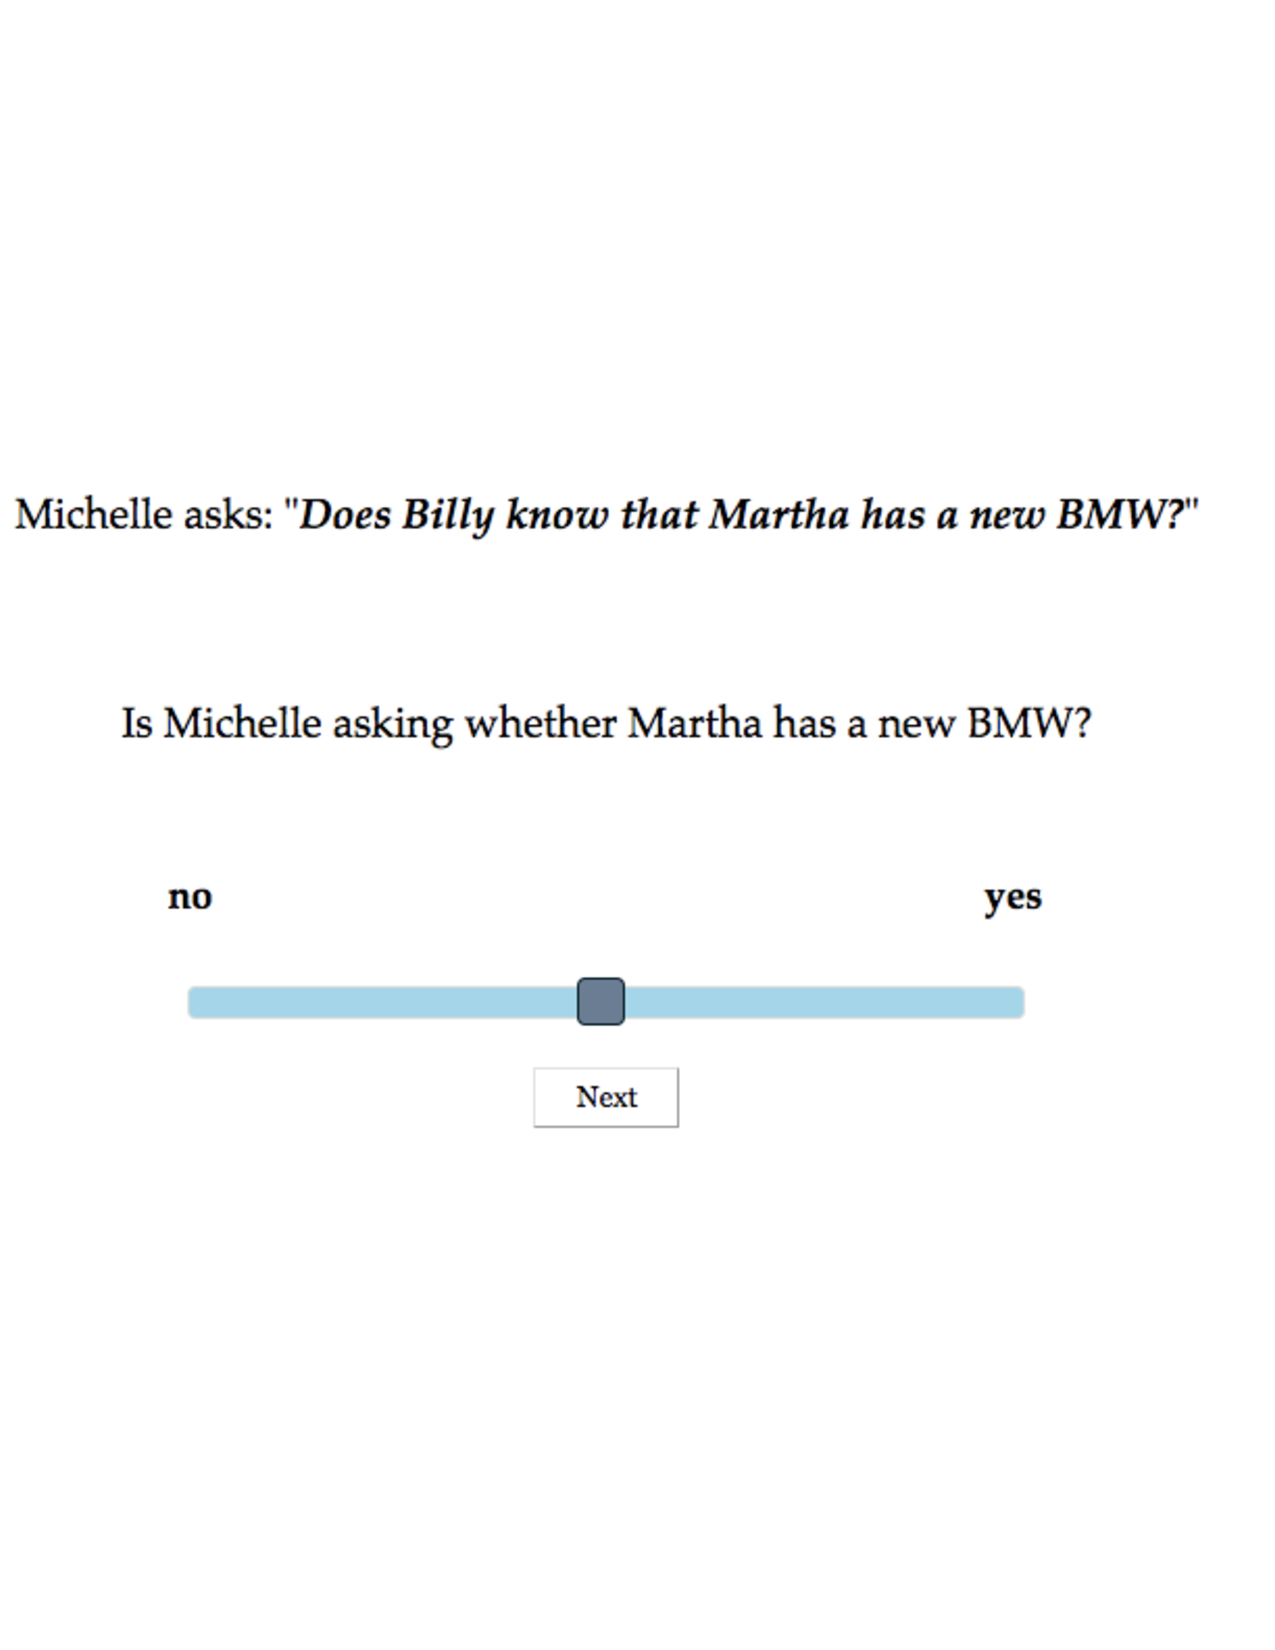
\includegraphics[width=12cm]{figures/exp1-trial}}
\end{center}
\caption{A sample (at-issueness) trial in Experiment 1a}\label{f-trial-exp1}
\end{figure}

A `yes' response to a `certain that' question was taken to indicate that the person who uttered the polar question (e.g., Michelle in the sample trial) was committed to the relevant lexical content, i.e., that the lexical content projects, whereas a `no' response was taken to indicate that the lexical content did not project. For the `asking whether' questions, a `yes'  response was taken to indicate that the speaker was asking about the relevant lexical content, i.e., that it was at-issue, whereas a `no' response was taken to indicate that the lexical content was not at-issue. To explore the hypothesis that projectivity and not-at-issueness are positively related,  `yes' responses to `certain that' questions and `no' responses to `asking whether' questions were coded as 1; `no' responses to `certain that' questions and `yes' responses to `asking whether' questions were coded as 0.

After completing the experiment, participants filled out a short optional survey about their age, their native language(s) and, if English is their native language, whether they are a speaker of American English (as opposed to, e.g., Australian or Indian English). To encourage them to respond truthfully, participants were told that they would be paid no matter what answers they gave in the survey.

\paragraph{Data exclusion.}
Prior to analysis, the data from 29 participants who did not self-identify as native speakers of American English were excluded. For the remaining 221 participants, we inspected their response means to the `certain that' and `asking whether' questions 
to the main clause controls: for these stimuli, we expect low responses to both types of questions since main clause contents are expected to be at-issue and not project. The response means of 11 participants were more than 3 standard deviations above the group means for at least one type of question (the group means were 0.07 for `certain that' and 0.04 for `asking whether' questions). Closer inspection revealed that these participants' responses to the control polar questions were systematically higher than the group means and involved 16 of the 17 contents, suggesting that these participants did not attend to the task or interpreted the task differently. The data from these 11 participants were also excluded, leaving data from 210 participants (ages 19-68; median: 33).  


\subsubsection{Results}

We begin by addressing the two main questions of interest, namely whether there is projection variability across target expressions and whether projectivity a function of at-issueness, as predicted by the Projection Principle. By-expression variability can be seen in \figref{fig:proj-triggmeans}:  while median projectivity ratings were all close to ceiling (suggesting that for each projective content at least half of the participants took it to be robustly projective), the variable mean responses, box sizes and whisker lengths provide evidence of variability in projectivity across target expressions. For example, mean projectivity of of the prejacent of \emph{only} was relatively low at .76, while mean projectivity of the projective contents of NRRCs and \emph{annoyed} was close to ceiling at .96. \figref{fig:proj-subjmeans} shows that about one third of participants took the 9 projective contents they judged to be robustly projective. For the remaining participants, the decreasing means (from right to left) reveal a decrease in the overall projectivity of the 9 projective contents and the increasingly larger error bars reveal an increase in projection variability among the 9 projective contents. 

\jt{I will fix x-axis label of upper panel}

\begin{figure}[!h]
\centering

\subfloat[][Boxplot of projection variability by target expression, collapsing across lexical contents. Blue dots indicate trigger means and notches indicate medians.]{ 
	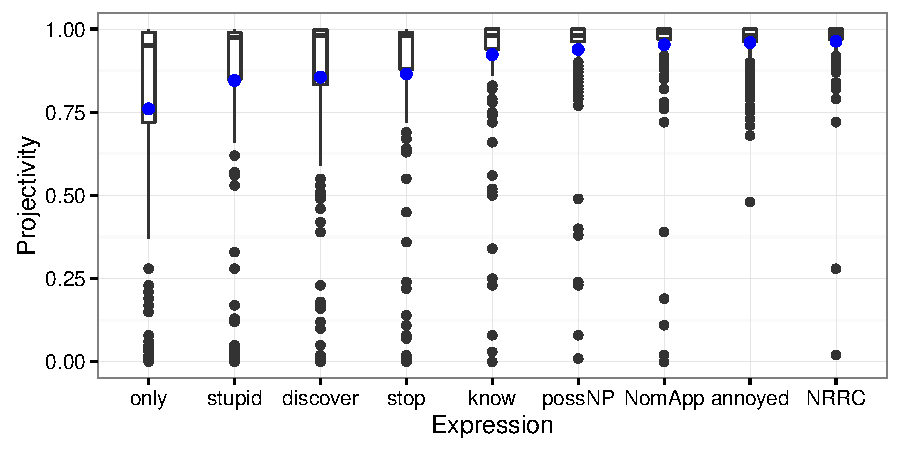
\includegraphics[width=12cm]{../results/exp1a/graphs/boxplot-projection}
	\label{fig:proj-triggmeans}
}

\subfloat[][Projectivity means by participant. Error bars indicate bootstrapped 95\% confidence intervals.]{ 
	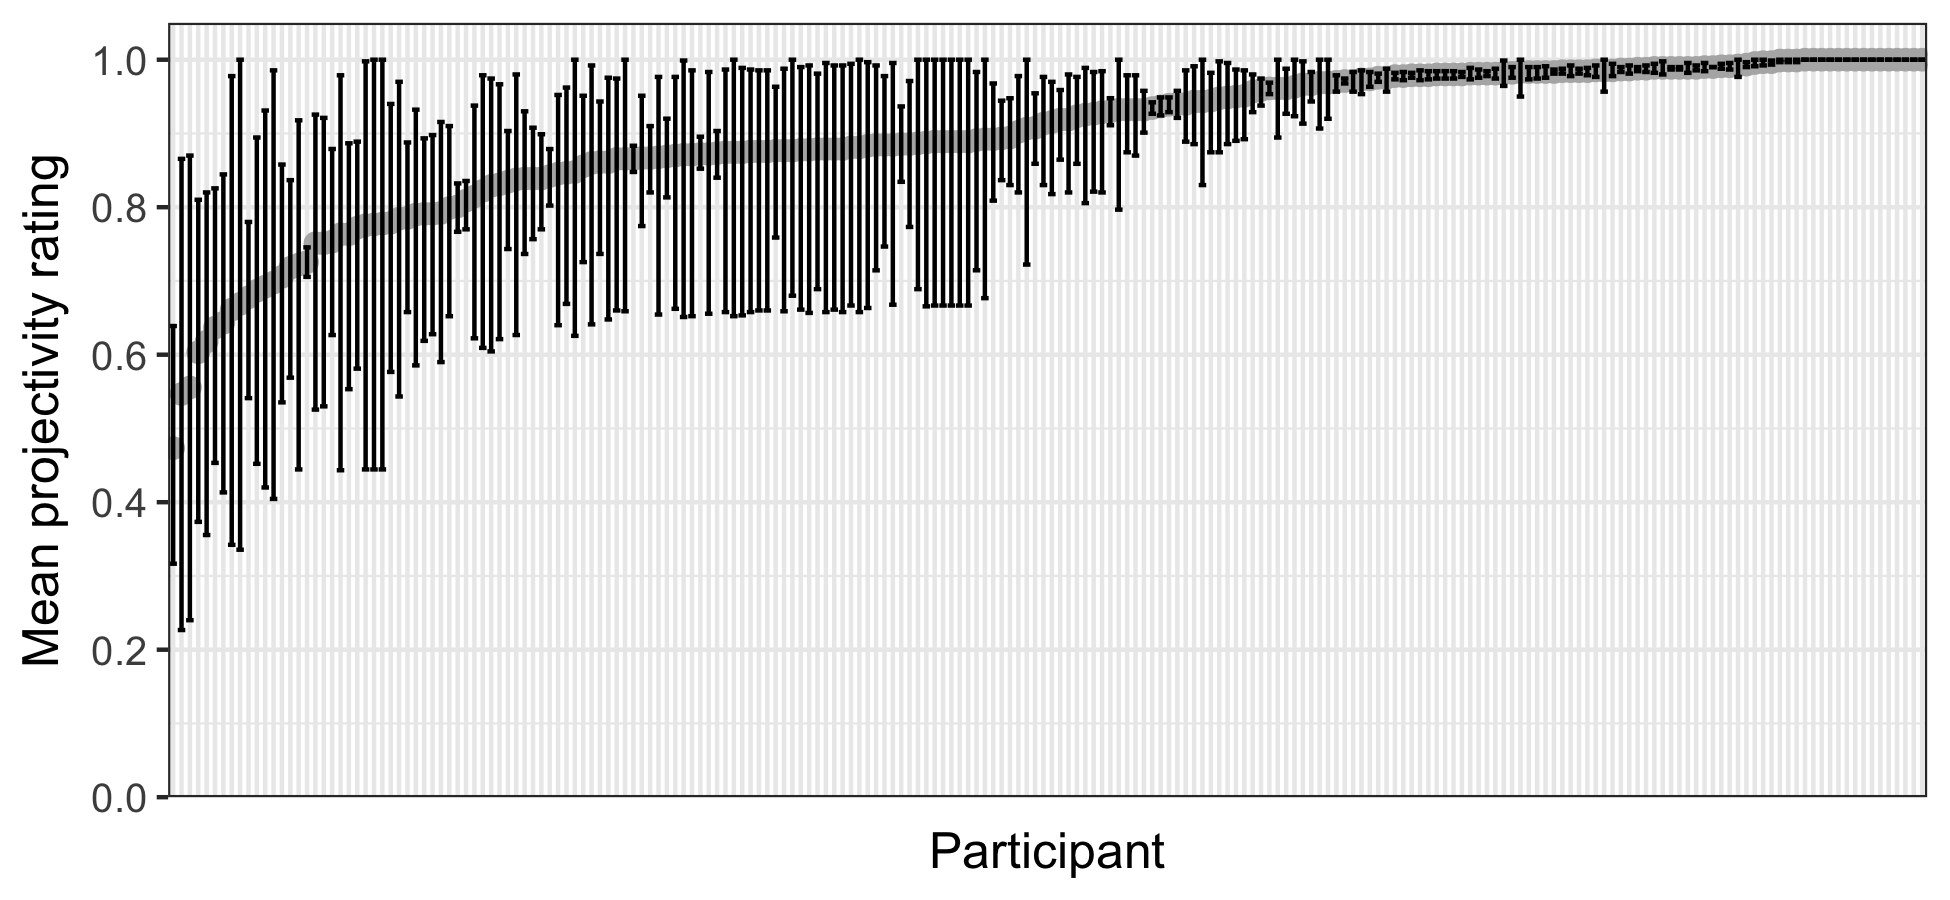
\includegraphics[width=12cm]{../results/exp1a/graphs/projection-subjectmeans}
	\label{fig:proj-subjmeans}
	}
	

\caption{Projectivity by target expression (top panel) and by participant (bottom panel)}
\label{fig:f-proj-1a}
\end{figure}


Mean projectivity ratings for the lexical contents that each target expression was paired with are visualized as a function of their mean not-at-issueness ratings in \figref{fig:f-proj-ai-1a}. There is a clear relationship between at-issueness and projectivity: lexical contents that received lower projectivity ratings are also lexical contents that participants considered to be more at-issue. \figref{fig:f-proj-ai-1a} also reveals projection variability between the lexical contents of each projective content trigger. 

\begin{figure}[!h]

\begin{center}
\includegraphics[width=12cm]{../results/exp1a/graphs/ai-proj-bytrigger-nofacets}
\end{center}

\caption{Mean projectivity against mean not-at-issueness by target expression and lexical content. Error bars indicate bootstrapped 95\% confidence intervals.}
\label{fig:f-proj-ai-1a}
\end{figure}

These qualitative observations about projection variability and the relation between at-issueness and projectivity are borne out statistically. We conducted a mixed-effects linear regression predicting projectivity rating from a centered fixed effect of at-issueness rating.\jt{JD, provide details on the function/package you used?} In order to control for block order effects, the model also included a centered fixed effect of block order. The model included the maximal random effects structure justified by the data and the theoretical questions: random by-expression intercepts (capturing differences in projectivity between target expressions),  random by-content intercepts (capturing differences in projectivity between lexical contents), random by-participant intercepts (capturing individual variability in projectivity), and random slopes for at-issueness by target expression, lexical content, and participant (capturing that the effect of at-issueness may vary across target expressions, lexical contents, and participants).  P-values were obtained by remove-one model comparison. The analysis was only conducted on non-main-clause trials, since we are specifically interested in variability in projectivity for contents that have the potential to project. 

There was a significant main effect of at-issueness such that more not-at-issue items received higher projectivity ratings ($\beta$ = 0.37, $SE$ = 0.16, $t$ = 3.48, $p <$ .006). This finding suggests that the information-structural status of a projective content is related to its projectivity, as predicted by the Projection Principle. 
Stepwise model comparison revealed that each random effect was justified, suggesting that there was by-participant, by-expression and by-content variability in projectivity, as well as variability in the at-issueness effect across participants, target expressions, and lexical contents. This finding suggests that there are target expression-specific, conventional, effects in projectivity. The block effect did not reach significance ($\beta$ = -0.01, $SE$ = 0.01, $t$ = -1.20, $p >$ .23), suggesting that the order in which participants completed the tasks (projectivity, at-issueness) did not affect their judgments in a systematic way.\jt{JD, include info about random effects.}

We conducted Bonferroni-corrected pairwise comparisons between triggers.\jt{JD, provide details on what function/package you used.} The results, displayed in \tableref{tab:pairwise}, suggest no difference in the projectivity of the projective contents of NRRCs, \emph{annoyed}, nominal appositives, possessive NPs, and \emph{know}. The projective contents of the other triggers differed from each other in projectivity, except for the pairs \emph{know/stop}, \emph{stop/discover}, \emph{stop/stupid} and \emph{discover/stupid}. However, the details of these differences between projective content triggers need to be taken with a grain of salt: since the triggers differed in the contents with which they occurred, and the regression analysis suggests that there is projection variability by content, these differences may not be due merely to differences between triggers but also to differences between contents.


\begin{table}[!h]
\begin{center}
\begin{tabular}{l l l l l l l l l}
\toprule
 &   NRRC & annoyed & NomApp &  possNP &  know & stop & discover & stupid \\
 \midrule
annoyed &  1.0  &  -  &        -   &       -  &        -  &   - &     -   &  -\\     
NomApp  &  1.0 & 1.0 & -    &   -   &    -    &   -  &     -   & - \\    
possNP  &    1.0 & 1.0 & 1.0 & - &      -  &     -     &  -   & - \\    
know     &   1.0 & 1.0 & 1.0 & 1.0 & -   &    -   &    -       & -\\
stop     &   8.9e-05 & 0.00023 & 0.00099 & 0.01568 & 0.19037 & - &  - & -\\      
discover  &   9.1e-06 & 2.6e-05 & 0.00013 & 0.00265 & 0.04359 & 1.0 & - & -      \\
stupid    &  6.3e-07 & 2.0e-06 & 1.1e-05 & 0.00031 & 0.00719 & 1.0 & 1.0 & - \\
only      &  $<$ 2e-16 & $<$ 2e-16 & $<$ 2e-16 & 1.1e-15 & 3.7e-13 & 2.2e-05 & 0.00020 & 0.00174 \\
\bottomrule
\end{tabular}

\caption{P-values associated with Bonferroni-corrected paired t-tests on trigger projectivity means.\jd{need to clean up this table if we want to keep it, but too tired right now} \jt{Rather than writing numbers in the table, can we just use * and ** and *** to indicate significance levels? Might be easier to read.}}
\label{tab:pairwise}
\end{center}
\end{table}

%
%\begin{figure}[!h]
%\begin{center}
%
%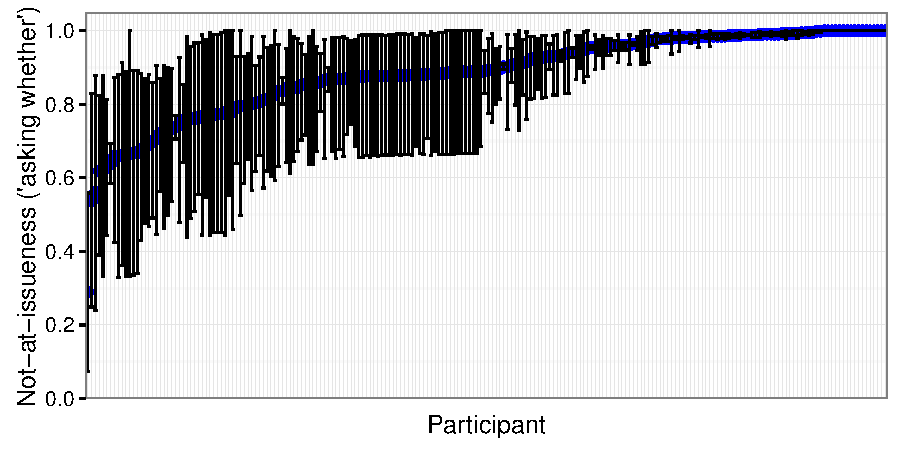
\includegraphics[width=12cm]{../results/exp1a/graphs/ai-subjectmeans}
%
%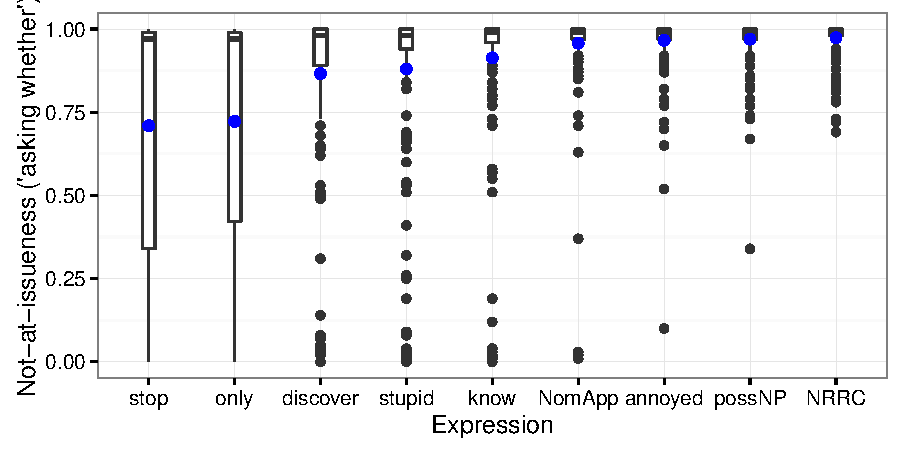
\includegraphics[width=12cm]{../results/exp1a/graphs/boxplot-not-at-issueness}
%
%\end{center}
%\caption{At-issueness by participant (top panel) and projective content trigger (bottom panel) \jd{not sure this is an interesting plot}}
%\label{f-ai-1a}
%\end{figure}
%
%


\subsubsection{Discussion}\label{s-discussion1a}

Experiment 1a was designed to explore projection variability for projective contents associated with a set of syntactically heterogeneous target expressions and to test a prediction of the Projection Principle, namely that the information-structural status of projective content is related to its projectivity. The experiment provided robust empirical evidence for variability in the extent to which the 9 projective contents project. Furthermore, the experiment provided empirical evidence for projection variability across participants. This finding suggests that speakers of American English differ in the extent to which they take the projective contents associated with the 9 target expressions to project. Finally, the experiment also showed that the lexical content that instantiates a projective content influences the extent to which the projective content projects. A methodological implication of these latter two findings is that research on projective content must be sensitive to potential differences in how robustly individual speakers judge projection and to the specific lexical content that instantiates a projective content.

The experiment also provided empirical support for the Projection Principle since the at-issueness of projective content was a significant predictor of its projectivity. This finding suggests that the extent to which a speaker is taken to be committed to a particular projective content is related to the extent to which the projective content is at-issue in the speaker's utterance. The experiment also provided empirical evidence that the target expressions differ in the extent to which the projective content they are associated with projects. This finding suggests that both the information-structural status of the projective content and the conventional meaning of the target expressions may play a role the extent to which a speaker is taken to be committed to a projective content.


\subsection{Experiment 1b}\label{s-exp1b} 

Experiment 1b was designed to explore the projectivity and at-issueness of the projective contents of the 12 predicates in (\ref{pairs1b2b}), i.e., the contents of the complements of the emotive factives ({\em be amused, be annoyed}), the cognitive factives ({\em know, be aware}), sensory factives ({\em see}), cognitive semi-factives ({\em discover, find out, realize, learn, establish}) and the communication semi-factives ({\em confess, reveal}).

\subsubsection{Methods}

\paragraph{Materials.} The 12 projective contents explored in this experiment were instantiated by the 20 lexical contents shown in (\ref{contents2}). Each of the 12 projective contents was instantiated by each of these 20 lexical contents, for a total of 200 target stimuli. 

\begin{exe}
\ex\label{contents2} 20 lexical contents in Experiment 1b 

\begin{enumerate}[itemsep=-.5mm]

\begin{multicols}{2}
\item Raul was drinking chamomile tea
\item Jack played frisbee with the kids
\item John was hiding in the garage
\item Mike visited the zoo
\item Zach dyed his hair purple
\item Marissa brought almond cupcakes
\item Chad put up a swing in his backyard
\item Greg drove his car into a ditch
\item Kate fell from her horse
\item Joyce got a poodle 
\columnbreak
\item Carl wrote a poem for his wife
\item Bea posted a family picture on Facebook
\item Janet moved into a damp apartment
\item Samantha bought a fur hat
\item Don ate a chili dog
\item Mary was biting her nails
\item Richie jumped into the pool
\item Martha came in her new BMW
\item Ann was dancing in the corner
\item Sue was doing yoga in the yard
\end{multicols}
\end{enumerate}

\end{exe}

The target stimuli were (past and present tense)\footnote{Stimuli with {\em be amused, be aware} and {\em be annoyed} were realized in the present tense; stimuli with the other predicates were realized in the past tense.} polar questions formed from sentences with one of the 12 predicates, a clausal complement formed from one of the 20 lexical contents in  (\ref{contents2}) and a random proper name subject (the names used for the subjects did not occur in the clausal complements). Two sample target stimuli are given in (\ref{sample2}):

\begin{exe}
\ex\label{sample2}
\begin{xlist}
\ex Is Shirley aware that Raul was drinking chamomile tea?

\ex Did Samuel discover that Raul was drinking chamomile tea?
\end{xlist}
\end{exe}

The experiment also included 20 control stimuli, which were (past tense) polar questions formed from sentences conveying the 20 lexical contents in (\ref{contents2}); a sample control polar question is shown in (\ref{sample3}). The control stimuli were included to confront participants with contents that are neither projective nor at-issue, and to assess whether participants were attending to the task.

\begin{exe}
\ex\label{sample3} Was Raul drinking chamomile tea?
\end{exe}

For each participant, a set of 20 polar question stimuli was randomly created: each set contained a target polar question for each of the 12 target expressions (the projective content of each expression was instantiated by a unique lexical content) and 8 control polar questions (with unique lexical contents as well, for a total of 20 unique lexical contents from (\ref{contents2})). Each participants' 20 polar question stimuli were presented twice: once (in a random order) in the `certain that' block to assess projectivity, and once (in a random order) in the `asking whether' block to assess at-issueness. Thus, each participant responded to questions about 40 polar question stimuli. Block order was random across the participants.

\paragraph{Procedure.} The procedure of Experiment 1b was the same as for Experiment 1a, described in section \ref{s-methods-1a}, except that participants responded to 20 `certain that' and 20 `asking whether' questions. (There are more trials in Experiment 1b than in Experiment 1a because each participant judged the projectivity and at-issueness of 20  rather than 15 contents.)

\paragraph{Participants.} 250 participants with U.S.\ IP addresses and at least 97\% of previous HITs approved were recruited on Amazon's Mechanical Turk platform (ages: 18-74; median: 32). They were paid \$1 for participating in the experiment. 

\paragraph{Data exclusion.} Prior to analysis, we excluded the data from 3 participants who did not self-identify as native speakers of American English. For the remaining 247 participants, we inspected their response means to the `certain that' and `asking whether' questions to the main clause controls. The response means of 12 participants were more than 3 standard deviations above the group means for at least one type of question (the group means were 0.08 for `certain that' and 0.04 for `asking whether' questions). Further inspection revealed that these participants' responses to the control questions were systematically higher than the group means and involved all of the 20 lexical contents, suggesting that these participants did not attend to the task or interpreted the task differently. The data from these 12 participants were also excluded, leaving data from 235 participants (ages 18-74; median: 33).

\subsubsection{Results}

We begin by addressing the research question in (\ref{questions}a), whether the contents of the complements of the 12 target expressions vary in how robustly they project. By-expression variability can be seen in \figref{fig:proj-triggmeans-1b}.  The median projectivity ratings are at ceiling for most of the (semi-)factive predicates, suggesting that at least half of the participants took the content of their complements to be robustly projective. The exceptions are the predicates {\em established, confessed} and {\em revealed}, for which the medians are not at ceiling, suggesting that the speaker was less likely to be taken to be committed to the contents of the complements of these predicates than for the other 9 predicates. By-expression variability is also suggested by variable mean responses, box sizes and whisker lengths across the 12 predicates. \figref{fig:proj-subjmeans-1b} shows that relatively few participants took the contents of the complements of the 12 predicates to be robustly projective. Instead, the mean responses suggest that there is by-participant variability in how robustly the contents of the complements of the 12 predicates was taken to project.

\jt{I will fix the x-axis label of the upper plot}

\begin{figure}[!h]
\centering

\subfloat[][Boxplot of projection variability by target expression, collapsing across  lexical contents. Blue dots indicate means and notches indicate medians.]{ 
	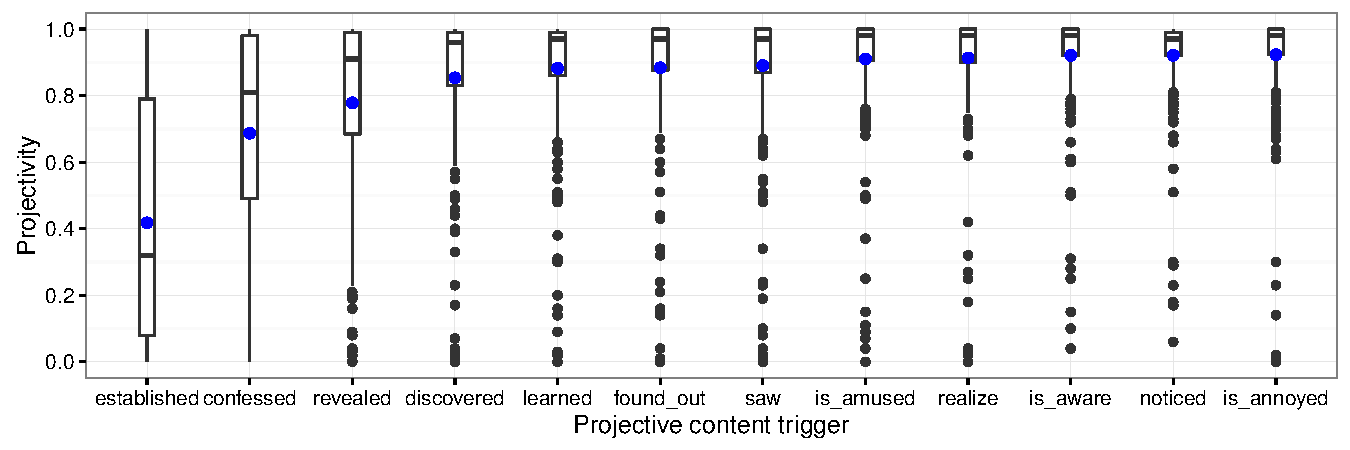
\includegraphics[width=16cm]{../results/exp1b/graphs/boxplot-projection}
	\label{fig:proj-triggmeans-1b}
}

\subfloat[][Projectivity means by participant. Error bars indicate bootstrapped 95\% confidence intervals.]{ 
	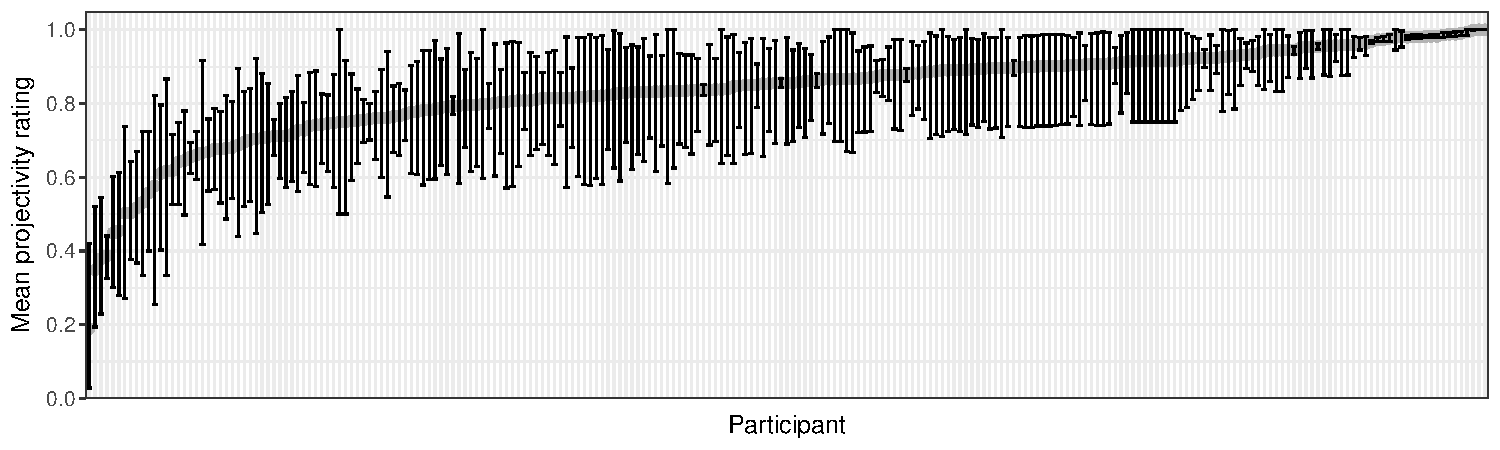
\includegraphics[width=16cm]{../results/exp1b/graphs/projection-subjectmeans}
	\label{fig:proj-subjmeans-1b}
	}
	

\caption{Projectivity by target expression (top panel) and by participant (bottom panel)}
\label{fig:f-proj-1b}
\end{figure}

\newpage

\jt{From here on I just copied the results section from Experiment 1a, in the hope that this makes completing this easier for you, JD}

Mean projectivity ratings for the lexical contents that each target expression was combined with are visualized as a function of their mean not-at-issueness ratings in \figref{fig:f-proj-ai-1b}. There is a clear relationship between at-issueness and projectivity: lexical contents that received lower projectivity ratings are also lexical contents that participants considered to be more at-issue. \figref{fig:f-proj-ai-1b} also reveals projection variability between the lexical contents of each of the 12 target expressions.

\begin{figure}[!h]

\begin{center}
\includegraphics[width=12cm]{../results/exp1b/graphs/ai-proj-bytrigger-nofacets}
\end{center}

\caption{Mean projectivity against mean not-at-issueness by target expression and lexical content. Error bars indicate bootstrapped 95\% confidence intervals.}
\label{fig:f-proj-ai-1b}
\end{figure}

These qualitative observations about projection variability and the relation between at-issueness and projectivity are borne out statistically. We conducted a mixed-effects linear regression predicting projectivity rating from a centered fixed effect of at-issueness rating.\jt{JD, provide details on the function/package you used?} In order to control for block order effects, the model also included a centered fixed effect of block order. The model included the maximal random effects structure justified by the data and the theoretical questions: random by-expression intercepts (capturing differences in projectivity between target expressions),  random by-content intercepts (capturing differences in projectivity between lexical contents), random by-participant intercepts (capturing individual variability in projectivity), and random slopes for at-issueness by target expression, lexical content, and participant (capturing that the effect of at-issueness may vary across target expressions, lexical contents, and participants).  P-values were obtained by remove-one model comparison. The analysis was only conducted on non-main-clause trials, since we are specifically interested in variability in projectivity for contents that have the potential to project. 

There was a significant main effect of at-issueness such that more not-at-issue items received higher projectivity ratings ($\beta$ = 0.XX, $SE$ = 0.XX, $t$ = XX, $p <$ XX). This finding suggests that the information-structural status of a projective content is related to its projectivity, in support of the Projection Principle. 
Stepwise model comparison revealed that each random effect was justified, suggesting that there was by-participant, by-expression and by-content variability, as well as variability in the at-issueness effect across participants, target expressions, and lexical contents. This finding suggests that there are expression-specific, conventional, effects in projectivity. The block effect did not reach significance ($\beta$ = XX, $SE$ = XX, $t$ = XX, $p >$ XX), suggesting that the order in which participants completed the tasks (projectivity, at-issueness) did not affect their judgments in a systematic way.\jt{JD, include info about random effects.}

We conducted Bonferroni-corrected pairwise comparisons between triggers.\jt{JD, provide details on what function/package you used.} The results, displayed in \tableref{tab:pairwise-1b}, suggest no difference in the projectivity of the projective contents \ldots. The projective contents of the other triggers differed from each other in projectivity\ldots. 

\jt{I can make this better, if we decide to keep this table, by tilting the top row 90 degrees}

\begin{table}[!h]
\begin{center}
\begin{tabular}{l l l l l l l l l l l l l}
\toprule
 &  established & confessed & revealed &  discovered &  learned & found out & saw & amused & realize & aware & noticed & annoyed \\
 \midrule
established & & & & & & & & & & & & \\ 
confessed & & & & & & & & & & & & \\ 
revealed & & & & & & & & & & & & \\ 
discovered & & & & & & & & & & & & \\ 
learned & & & & & & & & & & & & \\ 
found out & & & & & & & & & & & & \\ 
saw  & & & & & & & & & & & & \\ 
amused & & & & & & & & & & & & \\ 
realize  & & & & & & & & & & & & \\   
aware  & & & & & & & & & & & & \\ 
noticed    & & & & & & & & & & & & \\ 
annoyed   & & & & & & & & & & & & \\ 
\bottomrule
\end{tabular}

\caption{P-values associated with Bonferroni-corrected paired t-tests on trigger projectivity means.\jd{need to clean up this table if we want to keep it, but too tired right now} \jt{Rather than writing numbers in the table, can we just use * and ** and *** to indicate significance levels? Might be easier to read.}}
\label{tab:pairwise-1b}
\end{center}
\end{table}


%
%\begin{figure}[!h]
%\begin{center}
%
%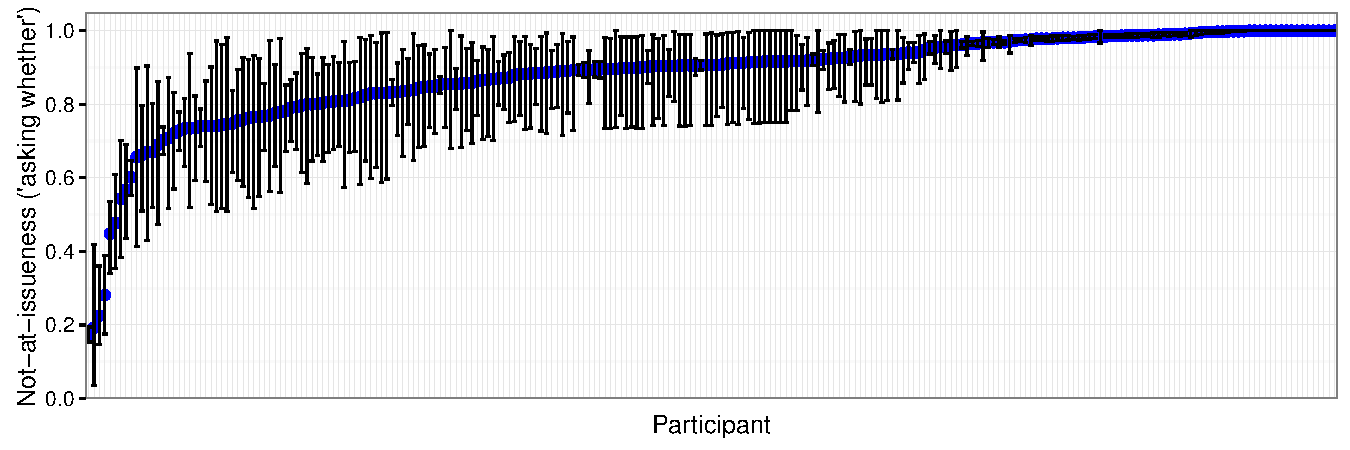
\includegraphics[width=16cm]{../results/exp1b/graphs/ai-subjectmeans}
%
%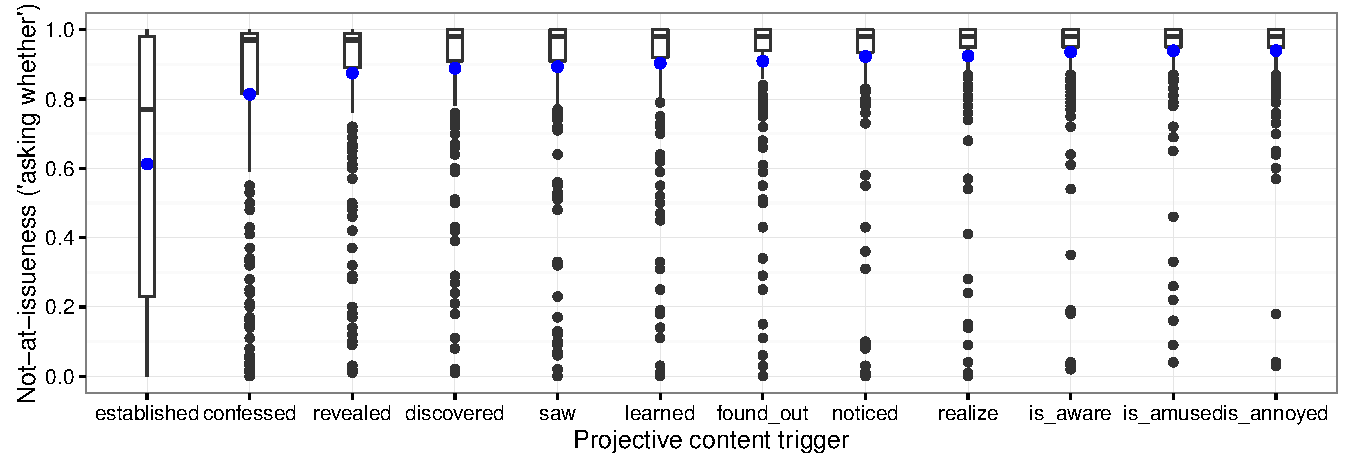
\includegraphics[width=16cm]{../results/exp1b/graphs/boxplot-not-at-issueness}
%
%\end{center}
%\caption{At-issueness by participant (top panel) and projective content trigger (bottom panel)}
%\label{f-ai-1b}
%\end{figure}

\jt{how do discover and annoyed compare in projectivity here, compared to Exp1a?}


\subsubsection{Discussion}

\jt{fill in, stopped revising here}

\subsection{Summary and discussion of Experiments 1a and 1b}

This paper set out to accomplish two goals, namely to explore projection variability for a broad range of projective content and to test the hypothesis put forth in \citealt{brst-salt10} and \citealt{brst-ar} that the projectivity of projective content is influenced by its information-structural status, specifically its at-issueness. Regarding the first goal, Experiments 1a and 1b have uncovered evidence for projection variability among the projective contents contributed by a set of 19 syntactically heterogeneous projective content triggers. This finding significant expands our understanding of projection variability from previous experimental research (\citealt{xue-onea11,smith-hall11}). As discussed in section \ref{s-discussion1a}, the observed between-participant and -item projection variability presents a challenge to conventionalist approaches to projection. 

Regarding the second goal, Experiments 1a and 1b have provided empirical evidence for the hypothesis that the information-structural status of projective content influences its projectivity (\citealt{brst-salt10,brst-ar}). Such empirical support was already suggested by \citet[180]{xue-onea11}, who, comparing the results of two separate pilot studies, pointed to ``a clear correlation between projection and not-at-issueness''. Since in our Experiments 1a and 1b projectivity and at-issueness was investigated using a within-participant and within-item design, the experimental findings not only provide empirical support for the hypothesis but also allow us to quantify the influence of not-at-issueness on projectivity, and to assess item- and participant-variability.

Our investigation of the second goal critically relied on exploring the at-issueness of projective content. The diagnostic we used for this purpose in Experiments 1a and 1b was chosen for two reasons: first, the diagnostic was used in previous research on at-issueness (e.g., \citealt{amaral-etal07,tonhauser-sula6}), and, second, the diagnostic is applicable for diagnosing at-issueness of projective content realized in polar questions. Since we wanted to explore both projectivity and at-issueness as within-participant and within-item factors, we needed a diagnostic for at-issueness that was suitable. However, a potential worry with the `asking whether' at-issueness diagnostic used in Experiments 1a and 1b is that it may be too closely related to the projection diagnostic. After all, if Patrick, after uttering the polar question in (\ref{stim}), is taken to be certain that Martha's new car is a BMW, then he is presumably not asking whether Martha's new car is a new BMW, and if he is not certain that Martha's new car is a BMW, then he may be more likely to be taken to ask whether Martha's new car is a BMW.\footnote{Of course, according to our hypothesis, projectivity is the flipside of at-issueness.}

\begin{exe}

\exi{(\ref{stim})} Patrick asks: {\em Was Martha's new car, a BMW, expensive?} 

\begin{xlist}
\ex `certain that' question: Is Patrick certain that Martha's new car is a BMW?

\ex `asking whether' question: Is Patrick asking whether Martha's new car is a BMW?

\end{xlist}

\end{exe}
Luckily, many different diagnostics have been used in the literature to diagnose at-issueness (e.g., \citealt{tonhauser-sula6}; for further discussion, see section \ref{s5}). In the second pair of experiments, Experiments 2a and 2b, explore the at-issueness of the projective contents of the first pair of experiments, Experiments 1a and 1b, respectively, using a different diagnostic for at-issueness, with the goal of thereby strengthening our findings about the second goal of the paper. 


\section{Confirming the influence of information structure on projectivity}\label{s4}

In the two experiments discussed in this section, Experiments 2a and 2b, the at-issueness of the projective contents explored in Experiments 1a and 1b, respectively, is explored using a different diagnostic for at-issueness. Whereas the diagnostic used in Experiments 1a and 1b relied on the assumption that the context set is more likely to be partitioned by at-issue content and its negation rather than not-at-issue content and its negation, the diagnostic used in Experiments 2a and 2b relies on the assumption that at-issue content is more likely to be the antecedent of a propositional anaphor than not-at-issue content (see, e.g., \citealt[54]{potts05} and \citealt{tonhauser-sula6}). The 3-turn discourse in (\ref{sure}) illustrates the diagnostic for the appositive content of nominal appositives: the speaker of the first turn (Fred) utters an indicative sentence with the relevant expression and the speaker of the second turn (Carla) responds with the question {\em Are you sure?}, which is taken to involve an elided propositional anaphor {\em that}, as in {\em Are you sure about that?}. The speaker of the third turn, who is identical to the speaker of the first turn, utters an indicative sentence in which the content to be diagnosed realizes the content of the complement of {\em sure}. 


\begin{exe}
\ex\label{sure} 
\begin{xlist}
\exi{Fred:} Martha’s new car, a BMW, was expensive.

\exi{Carla:} Are you sure?

\exi{Fred:} Yes, I am sure that Martha's new car is a BMW.
\end{xlist}

%\ex
%
%\begin{xlist}
%\exi{Sandra:} Billy discovered that Martha has a new BMW.
%
%\exi{Carl:} Are you sure?
%
%\exi{Sandra:} Yes, I am sure that Martha's new car is a BMW.
%\end{xlist}
%\end{xlist}
\end{exe}
To diagnose whether the elided propositional anaphor {\em that} in the second turn can be taken to target the relevant content, participants were asked whether the speaker of the first/third turn answered the question of the other speaker, e.g., in (\ref{sure}) whether Fred answered Carla's question. The assumption is that participants will take Fred to have responded to Carla's question if the relevant content can be taken to be the antecedent of the elided propositional anaphor in Carla's question, i.e., can be at-issue, and participants will take Fred to not have responded to Carla's question if the relevant content cannot be taken to be the antecedent of the elided propositional anaphor in  Carla's question, i.e., cannot be at-issue.

Thus, the at-issueness diagnostic used in Experiments 2a/2b differs from the one used in Experiments 1a/1b in several ways: i) the projective content triggers are realized unembedded in assertions rather than in polar questions; ii) the diagnostic relies on the assumption that at-issue and not-at-issue content differ in the extent to which it can be the antecedent of a propositional anaphor, rather than in the extent to which it and its negation partition the context set; and iii) participants were asked to judge the extent to which an utterance answered a question, rather than what a speaker is asking about.

If the information-structural status of projective content influences its projectivity, we expect the extent to which projective content is not-at-issue under this second diagnostic for at-issueness to also influence the projectivity of the content.

\subsection{Experiment 2a}

Experiment 2a explored the at-issueness of the 9 projective contents that were already explored in Experiment 1a (see section \ref{s-exp1a}) using the {\em Are you sure?} diagnostic, i.e., the content of NRRCs and nominal appositives, the possession implication of possessive noun phrases, the prejacent of {\em only} and {\em stupid}, the pre-state implication of {\em stop} and the contents of the complements of {\em annoyed, discover} and {\em know}.

\subsubsection{Methods}\label{s-methods-2a}

\paragraph{Materials.} Stimuli consisted of 3-turn discourses between two individuals, as (\ref{sure}). In the target stimuli, the first turn of each discourse consisted of an indicative sentence that realized one of the 9 projective content triggers. The 9 projective contents explored in Experiment 2a were instantiated by the same 17 contents as in Experiment 1a, as described in section \ref{s-methods-1a}. Thus, there were a total of 43 indicative sentences with projective content triggers that realized the first turn of the target stimuli. The second turn of the target stimuli consisted of a second speaker's {\em Are you sure?} question. In the third turn, the first speaker utters {\em Yes, I am sure that}, with the relevant projective content realized as the content of the complement of {\em sure}. 

As in Experiment 1a, an additional 17 control discourses were formed with sentences that realize the 17 contents, as shown in (\ref{sure2}).

\begin{exe}
\ex\label{sure2}
\begin{xlist}
\exi{Sandra:} Martha has a new BMW.

\exi{Carl:} Are you sure?

\exi{Sandra:} Yes, I am sure that Martha has a new BMW.
\end{xlist}
\end{exe}
As in Experiment 1a, a set of 15 stimuli was randomly created for each participant: each set contained a target stimulus for each of the 9 projective content triggers (each  instantiated by a unique content) and 6 control stimuli (with unique contents as well, for a total of 15 unique contents). The full set of stimuli of Experiment 2a is provided in Appendix \ref{a-exp1a-2a-stimuli}.

\paragraph{Procedure.} Participants were told to imagine that they are at a party and, upon walking into the kitchen, overhear a short conversation between two people. Participants were then presented with their 15 stimuli in random order and were asked to assess, for each stimulus, whether the speaker of the first/third turn answered the question of the speaker of the second turn. Participants gave their responses on a slider marked `no' at one end and `yes' at the other, as shown in Figure \ref{f-trial-exp2a}. A `yes' response was taken to indicate that the relevant content was taken to be the antecedent of the elided propositional anaphor, i.e., that the content was at-issue; a `no' response was taken to indicate that the relevant content was not taken to be the antecedent of the elided propositional anaphor, i.e., that the content was not at-issue.
After responding to the 15 stimuli, participants completed the same survey as in Experiment 1a.


\begin{figure}[!h]
\begin{center}
\fbox{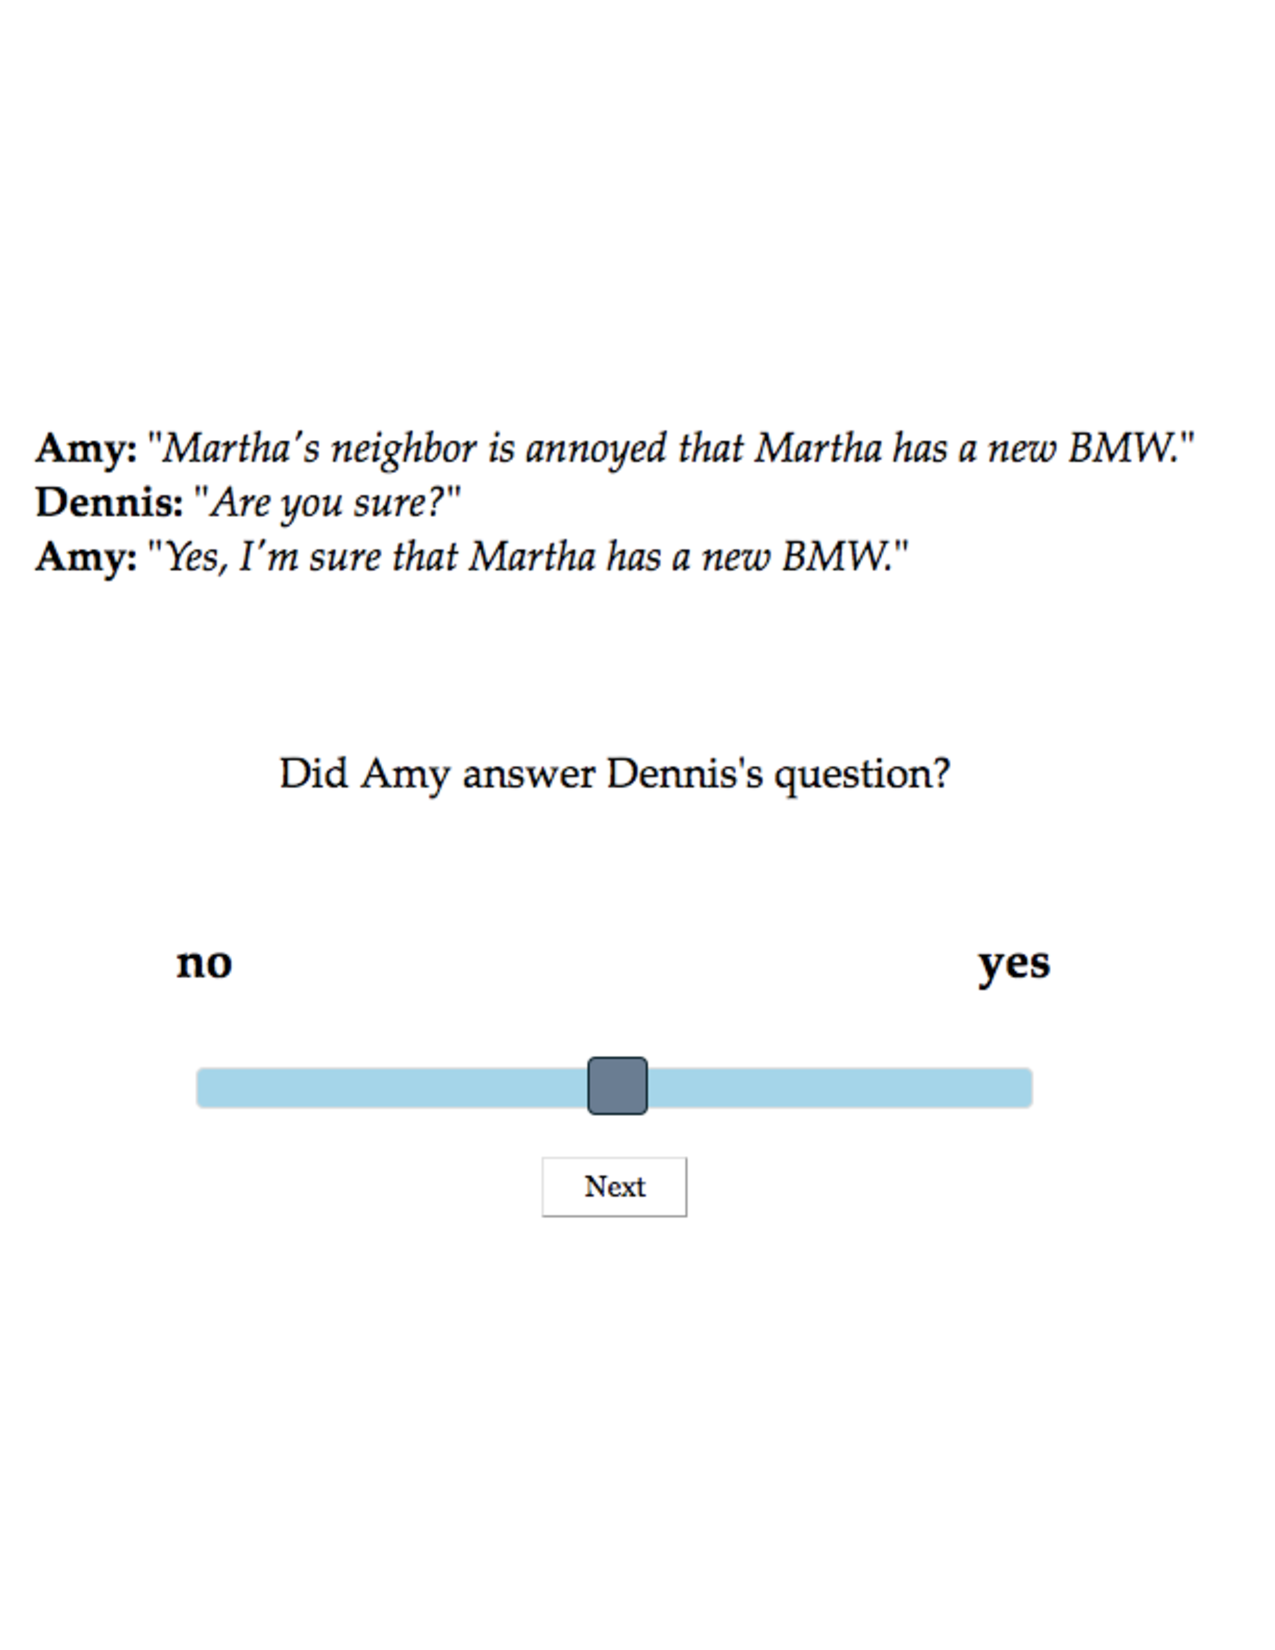
\includegraphics[width=12cm]{figures/exp2-trial}}
\end{center}
\caption{A sample trial in Experiment 2a}
\label{f-trial-exp2a}
\end{figure}

\paragraph{Participants.} 250 participants with U.S.\ IP addresses and at least 97\% of previous HITs approved were recruited on Amazon's Mechanical Turk platform (ages: 20-77; median: 30). They were paid 30 cents for their participation.

\subsubsection{Results}

The results about the relation between at-issueness and projectivity that are discussed in this section are based on the data from 238 participants (ages 20-77; median: 30). We excluded the data from 6 participants who did not self-identify as native speakers of American English. Inspection of the response means of the remaining 244 American-English speaking participants to the 6 control stimuli revealed 6 participants whose response means were more than 3 standard deviations above the group mean (which was 0.04). Further inspection revealed that these participants' responses were systematically higher than the group mean and involved 14 of the 17 contents, suggesting that these participants did not attend to the task or interpreted the task differently. The data from these 6 participants were also excluded.

\jt{analysis needed}


\begin{figure}[!h]
\begin{center}

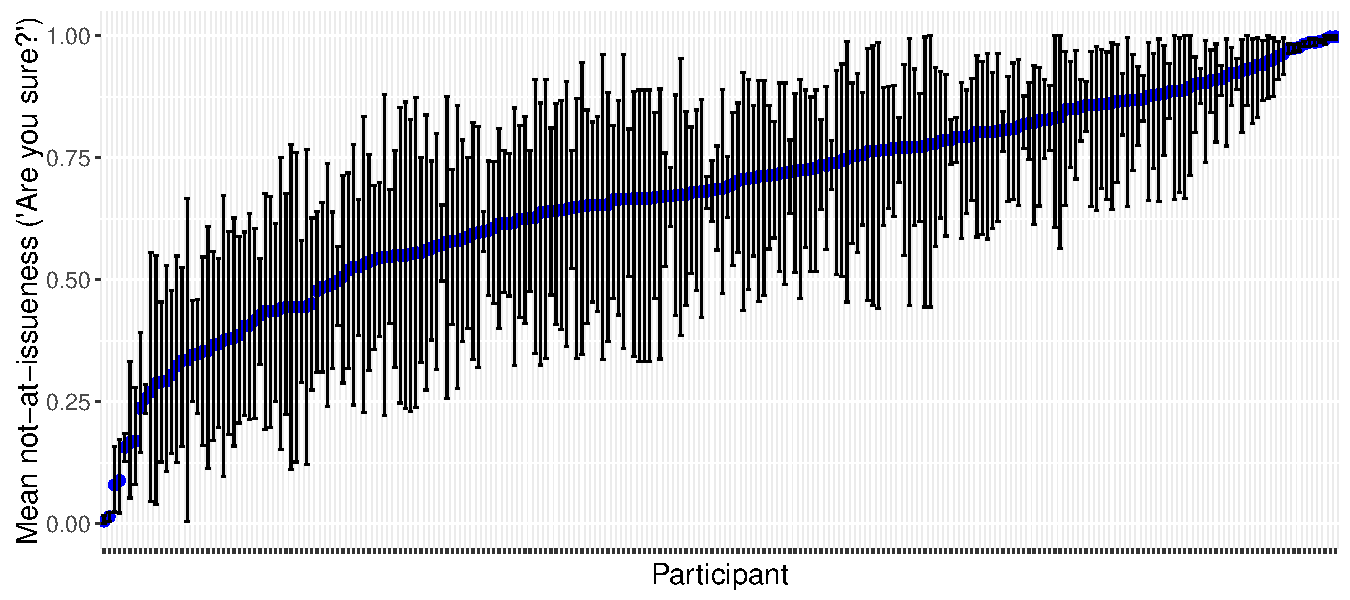
\includegraphics[width=12cm]{../results/exp2a/graphs/ai-subjectmeans}

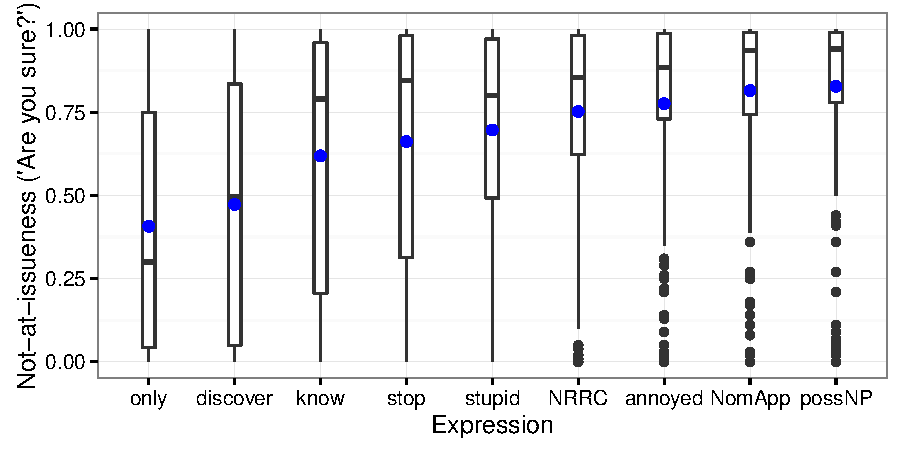
\includegraphics[width=12cm]{../results/exp2a/graphs/boxplot-not-at-issueness}

\end{center}
\caption{At-issueness by participant (top panel) and projective content trigger (bottom panel)}
\label{f-ai-2a}
\end{figure}



\subsubsection{Discussion}

\subsection{Experiment 2b} 

Experiment 2b was designed to explore, using the {\em Are you sure?} diagnostic, the at-issueness of the projective contents of the 12 predicates explored in Experiment 1b, i.e., the emotive factives {\em be amused} and {\em be annoyed}, the cognitive factives {\em know} and {\em be aware}, the sensory factive {\em see}, the cognitive semi-factives {\em discover, find out, realize, learn} and {\em establish} and the communication semi-factives {\em confess} and {\em reveal}.

\subsubsection{Methods}


\paragraph{Materials.} As in Experiment 2a, the stimuli consisted of 3-turn discourses between two individuals. In the target stimuli, the first turn of each discourse consisted of an indicative sentence that realized one of the 12 predicates, as shown in (\ref{sure3}). The contents of the complements of these predicates were instantiated by the same 20 contents as in Experiment 1b, as described in section \ref{s-methods-2a}. Thus, there were a total of 240 indicative sentences with projective content triggers that realized the first turn of the target stimuli. The second turn of the target stimuli consisted of a second speaker's {\em Are you sure?} question. In the third turn, the first speaker utters {\em Yes, I am sure that}, with the relevant projective content realized as the content of the complement of {\em sure}. 

\begin{exe}
\ex\label{sure3}
\begin{xlist}
\exi{Sandra:} Shirley is aware that Raul was drinking chamomile tea.

\exi{Carl:} Are you sure?

\exi{Sandra:} Yes, I am sure that Raul was drinking chamomile tea.
\end{xlist}
\end{exe}

As in Experiment 1b, an additional 20 control discourses were formed with sentences that realize the 20 contents, as shown in (\ref{sure4}).

\begin{exe}
\ex\label{sure4}
\begin{xlist}
\exi{Sandra:} Raul was drinking chamomile tea.

\exi{Carl:} Are you sure?

\exi{Sandra:} Yes, I am sure that Raul was drinking chamomile tea.
\end{xlist}
\end{exe}
As in Experiment 1b, a set of 20 stimuli was randomly created for each participant: each set contained a target stimulus for each of the 12 predicates (whose complements each was instantiated by a unique content) and 8 control stimuli (with unique contents as well, for a total of 20 unique contents). 

\paragraph{Procedure.} The procedure was the same as in Experiment 2a, described in section \ref{s-methods-2a}, except that participants responded to 20 stimuli, rather than just 15.

\paragraph{Participants.} 250 participants with U.S.\ IP addresses and at least 97\% of previous HITs approved were recruited on Amazon's Mechanical Turk platform (ages: 18-77; median: 29). They were paid 30 cents for their participation.

\subsubsection{Results}

The results about the relation between at-issueness and projectivity that are discussed in this section are based on the data from 238 participants (ages 18-77; median: 30). We excluded the data from 6 participants who did not self-identify as native speakers of American English. Inspection of the response means of the remaining 244 American-English speaking participants to the 8 control stimuli revealed 6 participants whose response means were more than 3 standard deviations above the group mean (which was 0.05). Further inspection revealed that these participants' responses were systematically higher than the group mean and involved 18 of the 20 contents, suggesting that these participants did not attend to the task or interpreted the task differently. The data from these 6 participants were also excluded.

\jt{analyses needed: at-issueness variability, influence of at-issueness on projectivity from Exp 1b}

\begin{figure}[!h]
\begin{center}

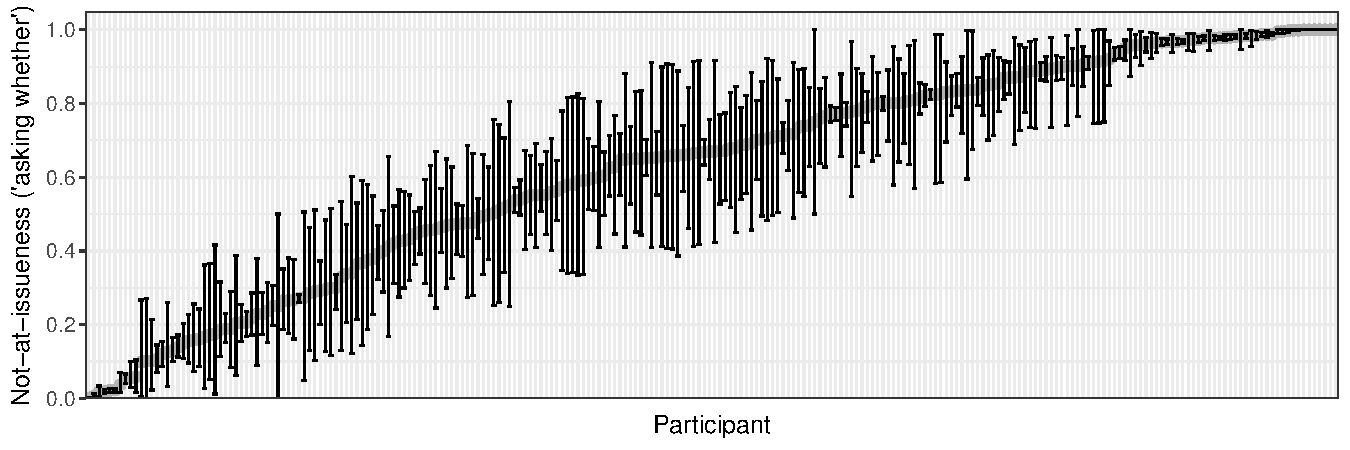
\includegraphics[width=16cm]{../results/exp2b/graphs/ai-subjectmeans}

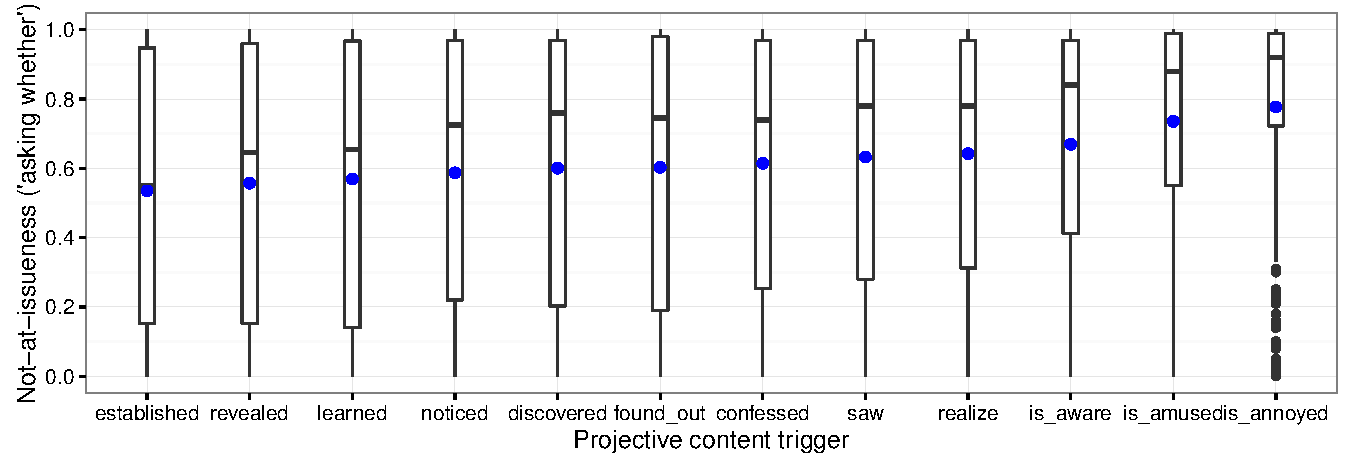
\includegraphics[width=16cm]{../results/exp2b/graphs/boxplot-not-at-issueness}

\end{center}
\caption{At-issueness by participant (top panel) and projective content trigger (bottom panel)}
\label{f-ai-2b}
\end{figure}

\subsubsection{Discussion}

\subsection{Summary and discussion of Experiments 2a and 2b}

\jt{analyses needed: relation between the at-issueness diagnostics in Experiments 1a/1b and Experiments 2a/2b}

\section{Discussion}\label{s5}

\begin{itemize}

\item Can theories of projection predict our findings (variability, relation to AIness)? We think our findings show that Projection Principle is true, and now discusses how that might come about.

\item This paper doesn't test whether triggering is conventional or not, though it is suggestive; we have the following hypothesis: conventional non-variability hypothesis says that for a conventional trigger you won't get variation in projectivity (implicit); under this hypothesis (which we don't test), the results do indeed mean that some triggers are conventional and others are not; make explicit under which conditions we can make which inferences

\begin{itemize}

\item Kartunen plugs holes filters: doesn't explain any cases where you don't get projection from a projection (variability, AI), embedding environment is crucial

\item Gazdar: you'll get projection unless you have a contradiction; no contradictions in our contexts; so again no explanation for our data; theory predicts robust projection

\item heim/vds: you'll get projection unless either there's a contradiction or a lack of informativeness; again, neither applies in our data, so they can't explain the data

\item Abusch:

\item Abrusan: 

\item Partee: information structure influences local accommodation (allegation and local accommodation)

\item Best question/SALT paper: suggest a hypothesis (extended projectivity hypothesis in AR paper), strong hypothesis that ainess inversely correlates with projectivity; we think that there's a mix of conventional and conversational triggering; we argue in BQ paper that you could do with only conversational trigger, but we haven't settled the case yet whether there is conventional triggering

\item Occam's Razor: conventional + accommodation, or only conversational


\end{itemize}

Under conventionalist approaches to projection, the projectivity of content is derived from a conventionally specified requirement that the content be entailed by or satisfied in the common ground prior to utterance (e.g., \citealt{heim83,vds92}). Thus, for instance, conventionally requiring that the contents of the complements of {\em discover} and {\em annoyed} are entailed by the common ground of the interlocutors prior to utterance derives the observation that the contents of the complements project over entailment-canceling operators. However, such approaches to projection do not lead us to expect that the contents of the complements of these two predicates differ in how robustly they project since, after all, the two contents receive the same conventional specification. Furthermore, such approaches to projection do not lead us to expect that two speakers of American English will differ in how robustly they take the content of the complement of {\em discover} to project since, again, the content of the complement of {\em discover} is conventionally specified to project for both speakers. Thus, our finding that there is both between-item and between-participant variability in how robustly projective content projects is an empirical challenge to conventional approaches to projection. \jd{i don't think that we can sell the strongest anti-conventionalist story, though, given that not all of the variability can be reduced to at-issueness (which we know from the fact that the by-trigger random effects were justified) -- though it's possible at least in principle that the trigger effects can be reduced to the particular contents they occurred with, we also included by-content random effects that ended up being justified in addition to the trigger random effects. That is, all these things are contributing independent variance.}

Conventionalist approaches are not helped here by appealing to local accommodation, the process by which projective content is accommodated in the scope of an entailment-canceling operator, e.g., to avoid contradictions, uninformativity or problems with binding (\citealt{heim83,vds92}). The context in which participants in Experiment 1a were asked to interpret the polar question stimuli was quite minimal since it only clarified that the participant overheard the speaker uttering the polar question upon entering the kitchen, at a party. Crucially, because the context was so minimal, the relevant projective contents cannot be argued to be locally accommodated to avoid contradictions with the context or to avoid uninformativity; and since the projective contents do not contain variables, problems with binding also do not warrant an appeal to local accommodation. Furthermore, in order for local accommodation to align conventionalist approaches to projection with the observed between-item and -participant variability, one would have to argue that, e.g., the content of the complement of {\em discover} is more likely to be locally accommodated than the content of the complement of {\em annoyed}, or that one participant is more likely to locally accommodate the content of the complement of {\em discover} than another participant. Absent a better understanding of local accommodation, such arguments are implausible. 

One way forward would be to develop a better understanding of local accommodation. Here we take a different route and suggest that the observed between-item and -participant variability provides empirical support for non-conventional approaches to projection, which attempt to derive projectivity from independently-motivated properties of projective content triggers and their use in context (e.g., \citealt{stalnaker74,kempson75,wilson75,boer-lycan76,levinson83,kadmon01,simons01,simons04,atlas05,abusch10,abrusan2011,best-question}). Under such approaches, between-item and -participant variability in projectivity could be attributed to differences between projective contents and their triggers. One such approach, as mentioned above, maintains that projective content differs in its information-structural properties, which has consequences for its projectivity: according to \citealt{brst-salt10} and \citealt{brst-ar}, projective content projects if and only if it is not at-issue. In Experiment 1a, the at-issueness of projective content was explored on the basis of a diagnostic for at-issueness that assumes that at-issue content differs from not at-issue content in how likely it (and its negation) are to partition the context set. The finding of Experiment 1a that the information-structural status of projective content, as diagnosed by this assumption about at-issueness, is a significant predictor of its projectivity provides empirical support the non-conventionalist approach to projection advanced in \citealt{brst-salt10} and \citealt{brst-ar}. In Experiment 1b, we extend our investigation of this hypothesis about projection to a wider range of projective content, namely the contents of the complements of (semi-)factive predicates.


At-issueness (DGfS talk, \citealt{tonhauser-dgfs2017}):

\begin{itemize}

\item At least 5 different assumptions are made about at-issueness in at-issueness diagnostics that are currently being used in the literature.

\item We have used two diagnostics here that rely on distinct assumptions about at-issueness (partition, anaphoricity). Both revealed an influence of at-issueness on projectivity.

\item But we have also observed that the two diagnostics lead to slightly different findings about at-issueness:

\begin{itemize}

\item e.g., {\em discover} versus {\em stop} (others?)

\item generally higher at-issueness in `are you sure?' diagnostic than in `asking whether' diagnostic suggests that projective content may be more available as antecedent to anaphor than be able to partition the context set

\end{itemize}

\item Furthermore, in a different experimental investigation, \citealt{syrett-koev2015} investigate the at-issueness of NRRCs and nominal appositives using the assent/dissent assumption (though that also involves propositional anaphora). They find that at-issueness depends on position and type. But just numerically, their results are more like our `are you sure?' diagnostic than our `asking whether' diagnostic.

\item Clearly an important topic for future research: i) what's a formal characterization of at-issueness? ii) which properties of at-issue and not-at-issue content derive from this formal characterization? iii) how can these properties be diagnosed with theoretically untrained speakers? 

\end{itemize}


\section{Conclusions}\label{s6}

\appendix

\section{Stimuli used in Experiments 1a and 2a}\label{a-exp1a-2a-stimuli}

The stimuli used in Experiments 1a are grouped here by the 17 instantiating contents. For each content, the first line provides the identifier of the content (e.g., `muffins', for the first content). The second line (`Content') identifies the content that instantiated the projective contents of the relevant projective content triggers. The remaining lines of each of the 17 contents identify the projective content triggers that were instantiated by the content (e.g., `muffins' instantiated control stimuli, NRRCs and {\em only}). In Experiment 2a, indicative sentence variants of the polar questions were used.

\begin{enumerate}

\item  muffins:  \\
     Content: these muffins have blueberries in them\\
     Control stimulus: Do these muffins have blueberries in them?\\
     NRRC: Are these muffins, which have blueberries in them, gluten-free and low-fat?\\
     {\em only}: Do these muffins only have blueberries in them?

\item pizza:  \\
     Content: this pizza has mushrooms on it\\
     Control stimulus: Does this pizza have mushrooms on it?\\
     {\em only}: Does this pizza only have mushrooms on it?\\
     {\em annoyed}: Is Sam annoyed that this pizza has mushrooms on it?\\
     {\em discover}: Did Sam discover that this pizza has mushrooms on it?

\item play:  \\
     Content: Jack was playing outside with the kids\\
     Control stimulus: Was Jack playing outside with the kids?\\
     {\em stop}: Did Jack stop playing outside with the kids?\\
     {\em know}: Does Daria know that Jack was playing outside with the kids?\\
     {\em discover}: Did Paula discover that Jack was playing outside with the kids?

\item veggie:  \\
     Content: Don is a vegetarian\\
     Nominal appositive: Is Don, a vegetarian, going to find something to eat here?\\
     NRRC: Is Don, who is a vegetarian, going to find something to eat here?\\
     Control stimulus: Is Don a vegetarian?

\item cheat:  \\
     Content: Raul cheated on his wife\\
     Control stimulus: Did Raul cheat on his wife?\\
     {\em know}: Does Daria know that Raul cheated on his wife?\\
     {\em stupid}: Was Raul stupid to cheat on his wife?

\item nails:  \\
     Content: Mary's daughter has been biting her nails\\
     Control stimulus: Has Mary's daughter been biting her nails?\\
     {\em discover}: Did Mary discover that her daughter has been biting her nails?\\
     {\em stop}: Has Mary's daughter stopped biting her nails?\\
     {\em stupid}: Is Mary's daughter stupid to be biting her nails?

\item  ballet:  \\
     Content: Ann used to dance ballet\\
     Control stimulus: Did Ann use to dance ballet?\\
     Nominal appositive: Is Ann, a former ballet dancer, limping?\\
     {\em stop}: Did Ann stop dancing ballet?

\item kids:  \\
     Content: John's kids were in the garage\\
     {\em only}: Were John's kids only in the garage?\\
     Control stimulus: Were John's kids in the garage?\\
     {\em stupid}: Were John's kids stupid to be in the garage?

\item hat:  \\
     Content: Samantha has a new hat\\
     Control stimulus: Does Samantha have a new hat?\\
     Possessive NP: Was Samantha's new hat expensive?\\
     {\em know}: Does Daria know that Samantha has a new hat?\\
     {\em annoyed}: Is Joyce annoyed that Samantha has a new hat?

\item bmw:  \\
     Content: Martha has a new BMW\\
     Control stimulus: Does Martha have a new BMW?\\
     Possessive NP: Was Martha's new BMW expensive?\\
     Nominal appositive: Was Martha's new car, a BMW, expensive?\\
     {\em annoyed}: Is Martha's neighbor annoyed that Martha has a new BMW?\\
     {\em know}: Does Billy know that Martha has a new BMW?

\item boyfriend:  \\
     Content: Betsy has a boyfriend\\
     Control stimulus: Does Betsy have a boyfriend?\\
     NRRC: Is Betsy, who has a boyfriend, flirting with the neighbor?\\
     Possessive NP: Is Betsy's boyfriend from around here?

\item alcatraz:  \\
     Content: Mike visited Alcatraz\\
     Control stimulus: Did Mike visit Alcatraz?\\
     NRRC: Is Mike, who visited Alcatraz, a history fan?\\
     {\em discover}: Did Jane discover that Mike visited Alcatraz?\\
     {\em know}: Does Jane know that Mike visited Alcatraz?

\item aunt:  \\
     Content: Janet has a sick aunt\\
     Control stimulus: Does Janet have a sick aunt?\\
     NRRC: Is Janet, who has a sick aunt, very compassionate?\\
     {\em know}: Does Melissa know that Janet has a sick aunt?\\
     Possessive NP: Has Janet's sick aunt been recovering?

\item cupcakes:  \\
     Content: Marissa brought the cupcakes\\
     Control stimulus: Did Marissa bring the cupcakes?\\
     NRRC: Is Marissa, who brought the cupcakes, a good baker?\\
     {\em know}: Does Max know that Marissa brought the cupcakes?

\item soccer:  \\
     Content: the soccer ball has a hole in it\\
     Control stimulus: Does the soccer ball have a hole in it?\\
     NRRC: Was the soccer ball, which has a hole in it, a gift from Uncle Bill?\\
     {\em annoyed}: Is Mandy annoyed that the soccer ball has a hole in it?\\
     {\em discover}: Did Mandy discover that the soccer ball has a hole in it?\\
     {\em know}: Does Mandy know that the soccer ball has a hole in it?

\item olives:  \\
   	Content: this bread has olives in it\\
   	Control stimulus: Does this bread have olives in it?\\
   	{\em annoyed}: Is Barbara annoyed that this bread has olives in it?

\item stuntman:  \\
   	Content: Richie is a stuntman\\
   	Control stimulus: Is Richie a stuntman?\\
   	Nominal appositive: Did Richie, a stuntman, break his leg?\\
   	{\em stupid}: Is Richie stupid to be a stuntman?

\end{enumerate}

\bibliographystyle{cslipubs-natbib}
\bibliography{bibliography}


\end{document}
